%Version 3 October 2023
% See section 11 of the User Manual for version history
%
%%%%%%%%%%%%%%%%%%%%%%%%%%%%%%%%%%%%%%%%%%%%%%%%%%%%%%%%%%%%%%%%%%%%%%
%%                                                                 %%
%% Please do not use \input{...} to include other tex files.       %%
%% Submit your LaTeX manuscript as one .tex document.              %%
%%                                                                 %%
%% All additional figures and files should be attached             %%
%% separately and not embedded in the \TeX\ document itself.       %%
%%                                                                 %%
%%%%%%%%%%%%%%%%%%%%%%%%%%%%%%%%%%%%%%%%%%%%%%%%%%%%%%%%%%%%%%%%%%%%%

%%\documentclass[referee,sn-basic]{sn-jnl}% referee option is meant for double line spacing

%%=======================================================%%
%% to print line numbers in the margin use lineno option %%
%%=======================================================%%

%%\documentclass[lineno,sn-basic]{sn-jnl}% Basic Springer Nature Reference Style/Chemistry Reference Style

%%======================================================%%
%% to compile with pdflatex/xelatex use pdflatex option %%
%%======================================================%%

%%\documentclass[pdflatex,sn-basic]{sn-jnl}% Basic Springer Nature Reference Style/Chemistry Reference Style


%%Note: the following reference styles support Namedate and Numbered referencing. By default the style follows the most common style. To switch between the options you can add or remove �Numbered� in the optional parenthesis. 
%%The option is available for: sn-basic.bst, sn-vancouver.bst, sn-chicago.bst%  
 
%%\documentclass[sn-nature]{sn-jnl}% Style for submissions to Nature Portfolio journals
%%\documentclass[sn-basic]{sn-jnl}% Basic Springer Nature Reference Style/Chemistry Reference Style
\documentclass[sn-mathphys-num]{sn-jnl}% Math and Physical Sciences Numbered Reference Style 
%%\documentclass[sn-mathphys-ay]{sn-jnl}% Math and Physical Sciences Author Year Reference Style
%%\documentclass[sn-aps]{sn-jnl}% American Physical Society (APS) Reference Style
%%\documentclass[sn-vancouver,Numbered]{sn-jnl}% Vancouver Reference Style
%%\documentclass[sn-apa]{sn-jnl}% APA Reference Style 
%%\documentclass[sn-chicago]{sn-jnl}% Chicago-based Humanities Reference Style

%%%% Standard Packages
%%<additional latex packages if required can be included here>

\usepackage{graphicx}%
\usepackage{multirow}%
\usepackage{amsmath,amssymb,amsfonts}%
\usepackage{amsthm}%
\usepackage{mathrsfs}%
\usepackage[title]{appendix}%
\usepackage{xcolor}%
\usepackage{textcomp}%
\usepackage{manyfoot}%
\usepackage{booktabs}%
\usepackage{algorithm}%
\usepackage{algorithmicx}%
\usepackage{algpseudocode}%
\usepackage{listings}%
\usepackage{tcolorbox}
\usepackage{tikz}
\usetikzlibrary{shapes.geometric}
\newcommand{\warningsign}{\tikz[baseline=-.75ex] \node[shape=regular polygon, regular polygon sides=3, inner sep=0pt, draw, thick] {\textbf{!}};}
\setlength{\parskip}{\baselineskip}

\definecolor{codegreen}{rgb}{0,0.6,0}
\definecolor{codegray}{rgb}{0.5,0.5,0.5}
\definecolor{codepurple}{rgb}{0.58,0,0.82}
% \definecolor{backcolour}{rgb}{0.95,0.95,0.92}
\definecolor{backcolour}{rgb}{1.0, 1.0, 1.0}

\lstdefinestyle{mystyle}{
		backgroundcolor=\color{backcolour},   
		commentstyle=\color{codegreen},
		keywordstyle=\color{magenta},
		numberstyle=\tiny\color{codegray},
		stringstyle=\color{codepurple},
		basicstyle=\ttfamily\footnotesize,
		breakatwhitespace=false,         
		breaklines=true,                 
		captionpos=b,                    
		keepspaces=true,                 
		numbers=left,                    
		numbersep=5pt,                  
		showspaces=false,                
		showstringspaces=false,
		showtabs=false,                  
		tabsize=2
}

\lstset{style=mystyle}
%%%%

%%%%%=============================================================================%%%%
%%%%  Remarks: This template is provided to aid authors with the preparation
%%%%  of original research articles intended for submission to journals published 
%%%%  by Springer Nature. The guidance has been prepared in partnership with 
%%%%  production teams to conform to Springer Nature technical requirements. 
%%%%  Editorial and presentation requirements differ among journal portfolios and 
%%%%  research disciplines. You may find sections in this template are irrelevant 
%%%%  to your work and are empowered to omit any such section if allowed by the 
%%%%  journal you intend to submit to. The submission guidelines and policies 
%%%%  of the journal take precedence. A detailed User Manual is available in the 
%%%%  template package for technical guidance.
%%%%%=============================================================================%%%%

%% as per the requirement new theorem styles can be included as shown below
\theoremstyle{thmstyleone}%
\newtheorem{theorem}{Theorem}%  meant for continuous numbers
%%\newtheorem{theorem}{Theorem}[section]% meant for sectionwise numbers
%% optional argument [theorem] produces theorem numbering sequence instead of independent numbers for Proposition
\newtheorem{proposition}[theorem]{Proposition}% 
%%\newtheorem{proposition}{Proposition}% to get separate numbers for theorem and proposition etc.

\theoremstyle{thmstyletwo}%
\newtheorem{example}{Example}%
\newtheorem{remark}{Remark}%

\theoremstyle{thmstylethree}%
\newtheorem{definition}{Definition}%

\raggedbottom
%%\unnumbered% uncomment this for unnumbered level heads

\begin{document}

\title[Article Title]{Article Title}

%%=============================================================%%
%% GivenName	-> \fnm{Joergen W.}
%% Particle	-> \spfx{van der} -> surname prefix
%% FamilyName	-> \sur{Ploeg}
%% Suffix	-> \sfx{IV}
%% \author*[1,2]{\fnm{Joergen W.} \spfx{van der} \sur{Ploeg} 
%%  \sfx{IV}}\email{iauthor@gmail.com}
%%=============================================================%%

\author*[1,2]{\fnm{First} \sur{Author}}\email{iauthor@gmail.com}

\author[2,3]{\fnm{Second} \sur{Author}}\email{iiauthor@gmail.com}
\equalcont{These authors contributed equally to this work.}

\author[1,2]{\fnm{Third} \sur{Author}}\email{iiiauthor@gmail.com}
\equalcont{These authors contributed equally to this work.}

\affil*[1]{\orgdiv{Department}, \orgname{Organization}, \orgaddress{\street{Street}, \city{City}, \postcode{100190}, \state{State}, \country{Country}}}

\affil[2]{\orgdiv{Department}, \orgname{Organization}, \orgaddress{\street{Street}, \city{City}, \postcode{10587}, \state{State}, \country{Country}}}

\affil[3]{\orgdiv{Department}, \orgname{Organization}, \orgaddress{\street{Street}, \city{City}, \postcode{610101}, \state{State}, \country{Country}}}

%%==================================%%
%% Sample for unstructured abstract %%
%%==================================%%

\abstract{The abstract serves both as a general introduction to the topic and as a brief, non-technical summary of the main results and their implications. Authors are advised to check the author instructions for the journal they are submitting to for word limits and if structural elements like subheadings, citations, or equations are permitted.}

%%================================%%
%% Sample for structured abstract %%
%%================================%%

% \abstract{\textbf{Purpose:} The abstract serves both as a general introduction to the topic and as a brief, non-technical summary of the main results and their implications. The abstract must not include subheadings (unless expressly permitted in the journal's Instructions to Authors), equations or citations. As a guide the abstract should not exceed 200 words. Most journals do not set a hard limit however authors are advised to check the author instructions for the journal they are submitting to.
% 
% \textbf{Methods:} The abstract serves both as a general introduction to the topic and as a brief, non-technical summary of the main results and their implications. The abstract must not include subheadings (unless expressly permitted in the journal's Instructions to Authors), equations or citations. As a guide the abstract should not exceed 200 words. Most journals do not set a hard limit however authors are advised to check the author instructions for the journal they are submitting to.
% 
% \textbf{Results:} The abstract serves both as a general introduction to the topic and as a brief, non-technical summary of the main results and their implications. The abstract must not include subheadings (unless expressly permitted in the journal's Instructions to Authors), equations or citations. As a guide the abstract should not exceed 200 words. Most journals do not set a hard limit however authors are advised to check the author instructions for the journal they are submitting to.
% 
% \textbf{Conclusion:} The abstract serves both as a general introduction to the topic and as a brief, non-technical summary of the main results and their implications. The abstract must not include subheadings (unless expressly permitted in the journal's Instructions to Authors), equations or citations. As a guide the abstract should not exceed 200 words. Most journals do not set a hard limit however authors are advised to check the author instructions for the journal they are submitting to.}

\keywords{keyword1, Keyword2, Keyword3, Keyword4}

%%\pacs[JEL Classification]{D8, H51}

%%\pacs[MSC Classification]{35A01, 65L10, 65L12, 65L20, 65L70}

\maketitle

\section{Introduction}\label{sec1}

% The Introduction section, of referenced text \cite{bib1} expands on the background of the work (some overlap with the Abstract is acceptable). The introduction should not include subheadings.

Springer Nature does not impose a strict layout as standard however authors are advised to check the individual requirements for the journal they are planning to submit to as there may be journal-level preferences. When preparing your text please also be aware that some stylistic choices are not supported in full text XML (publication version), including coloured font. These will not be replicated in the typeset article if it is accepted. 

\section{Results}\label{sec2}

Sample body text. Sample body text. Sample body text. Sample body text. Sample body text. Sample body text. Sample body text. Sample body text.

\section{This is an example for first level head---section head}\label{sec3}

\subsection{This is an example for second level head---subsection head}\label{subsec2}

\subsubsection{This is an example for third level head---subsubsection head}\label{subsubsec2}

Sample body text. Sample body text. Sample body text. Sample body text. Sample body text. Sample body text. Sample body text. Sample body text. 

\section{Equations}\label{sec4}

Equations in \LaTeX\ can either be inline or on-a-line by itself (``display equations''). For
inline equations use the \verb+$...$+ commands. E.g.: The equation
$H\psi = E \psi$ is written via the command \verb+$H \psi = E \psi$+.

For display equations (with auto generated equation numbers)
one can use the equation or align environments:
\begin{equation}
\|\tilde{X}(k)\|^2 \leq\frac{\sum\limits_{i=1}^{p}\left\|\tilde{Y}_i(k)\right\|^2+\sum\limits_{j=1}^{q}\left\|\tilde{Z}_j(k)\right\|^2 }{p+q}.\label{eq1}
\end{equation}
where,
\begin{align}
D_\mu &=  \partial_\mu - ig \frac{\lambda^a}{2} A^a_\mu \nonumber \\
F^a_{\mu\nu} &= \partial_\mu A^a_\nu - \partial_\nu A^a_\mu + g f^{abc} A^b_\mu A^a_\nu \label{eq2}
\end{align}
Notice the use of \verb+\nonumber+ in the align environment at the end
of each line, except the last, so as not to produce equation numbers on
lines where no equation numbers are required. The \verb+\label{}+ command
should only be used at the last line of an align environment where
\verb+\nonumber+ is not used.
\begin{equation}
Y_\infty = \left( \frac{m}{\textrm{GeV}} \right)^{-3}
    \left[ 1 + \frac{3 \ln(m/\textrm{GeV})}{15}
    + \frac{\ln(c_2/5)}{15} \right]
\end{equation}
The class file also supports the use of \verb+\mathbb{}+, \verb+\mathscr{}+ and
\verb+\mathcal{}+ commands. As such \verb+\mathbb{R}+, \verb+\mathscr{R}+
and \verb+\mathcal{R}+ produces $\mathbb{R}$, $\mathscr{R}$ and $\mathcal{R}$
respectively (refer Subsubsection~\ref{subsubsec2}).

\section{Tables}\label{sec5}

Tables can be inserted via the normal table and tabular environment. To put
footnotes inside tables you should use \verb+\footnotetext[]{...}+ tag.
The footnote appears just below the table itself (refer Tables~\ref{tab1} and \ref{tab2}). 
For the corresponding footnotemark use \verb+\footnotemark[...]+

\begin{table}[h]
\caption{Caption text}\label{tab1}%
\begin{tabular}{@{}llll@{}}
\toprule
Column 1 & Column 2  & Column 3 & Column 4\\
\midrule
row 1    & data 1   & data 2  & data 3  \\
row 2    & data 4   & data 5\footnotemark[1]  & data 6  \\
row 3    & data 7   & data 8  & data 9\footnotemark[2]  \\
\botrule
\end{tabular}
\footnotetext{Source: This is an example of table footnote. This is an example of table footnote.}
\footnotetext[1]{Example for a first table footnote. This is an example of table footnote.}
\footnotetext[2]{Example for a second table footnote. This is an example of table footnote.}
\end{table}

\noindent
The input format for the above table is as follows:

%%=============================================%%
%% For presentation purpose, we have included  %%
%% \bigskip command. Please ignore this.       %%
%%=============================================%%
\bigskip
\begin{verbatim}
\begin{table}[<placement-specifier>]
\caption{<table-caption>}\label{<table-label>}%
\begin{tabular}{@{}llll@{}}
\toprule
Column 1 & Column 2 & Column 3 & Column 4\\
\midrule
row 1 & data 1 & data 2	 & data 3 \\
row 2 & data 4 & data 5\footnotemark[1] & data 6 \\
row 3 & data 7 & data 8	 & data 9\footnotemark[2]\\
\botrule
\end{tabular}
\footnotetext{Source: This is an example of table footnote. 
This is an example of table footnote.}
\footnotetext[1]{Example for a first table footnote.
This is an example of table footnote.}
\footnotetext[2]{Example for a second table footnote. 
This is an example of table footnote.}
\end{table}
\end{verbatim}
\bigskip
%%=============================================%%
%% For presentation purpose, we have included  %%
%% \bigskip command. Please ignore this.       %%
%%=============================================%%

\begin{table}[h]
\caption{Example of a lengthy table which is set to full textwidth}\label{tab2}
\begin{tabular*}{\textwidth}{@{\extracolsep\fill}lcccccc}
\toprule%
& \multicolumn{3}{@{}c@{}}{Element 1\footnotemark[1]} & \multicolumn{3}{@{}c@{}}{Element 2\footnotemark[2]} \\\cmidrule{2-4}\cmidrule{5-7}%
Project & Energy & $\sigma_{calc}$ & $\sigma_{expt}$ & Energy & $\sigma_{calc}$ & $\sigma_{expt}$ \\
\midrule
Element 3  & 990 A & 1168 & $1547\pm12$ & 780 A & 1166 & $1239\pm100$\\
Element 4  & 500 A & 961  & $922\pm10$  & 900 A & 1268 & $1092\pm40$\\
\botrule
\end{tabular*}
\footnotetext{Note: This is an example of table footnote. This is an example of table footnote this is an example of table footnote this is an example of~table footnote this is an example of table footnote.}
\footnotetext[1]{Example for a first table footnote.}
\footnotetext[2]{Example for a second table footnote.}
\end{table}

In case of double column layout, tables which do not fit in single column width should be set to full text width. For this, you need to use \verb+\begin{table*}+ \verb+...+ \verb+\end{table*}+ instead of \verb+\begin{table}+ \verb+...+ \verb+\end{table}+ environment. Lengthy tables which do not fit in textwidth should be set as rotated table. For this, you need to use \verb+\begin{sidewaystable}+ \verb+...+ \verb+\end{sidewaystable}+ instead of \verb+\begin{table*}+ \verb+...+ \verb+\end{table*}+ environment. This environment puts tables rotated to single column width. For tables rotated to double column width, use \verb+\begin{sidewaystable*}+ \verb+...+ \verb+\end{sidewaystable*}+.

\begin{sidewaystable}
\caption{Tables which are too long to fit, should be written using the ``sidewaystable'' environment as shown here}\label{tab3}
\begin{tabular*}{\textheight}{@{\extracolsep\fill}lcccccc}
\toprule%
& \multicolumn{3}{@{}c@{}}{Element 1\footnotemark[1]}& \multicolumn{3}{@{}c@{}}{Element\footnotemark[2]} \\\cmidrule{2-4}\cmidrule{5-7}%
Projectile & Energy	& $\sigma_{calc}$ & $\sigma_{expt}$ & Energy & $\sigma_{calc}$ & $\sigma_{expt}$ \\
\midrule
Element 3 & 990 A & 1168 & $1547\pm12$ & 780 A & 1166 & $1239\pm100$ \\
Element 4 & 500 A & 961  & $922\pm10$  & 900 A & 1268 & $1092\pm40$ \\
Element 5 & 990 A & 1168 & $1547\pm12$ & 780 A & 1166 & $1239\pm100$ \\
Element 6 & 500 A & 961  & $922\pm10$  & 900 A & 1268 & $1092\pm40$ \\
\botrule
\end{tabular*}
\footnotetext{Note: This is an example of table footnote this is an example of table footnote this is an example of table footnote this is an example of~table footnote this is an example of table footnote.}
\footnotetext[1]{This is an example of table footnote.}
\end{sidewaystable}

\section{Figures}\label{sec6}

As per the \LaTeX\ standards you need to use eps images for \LaTeX\ compilation and \verb+pdf/jpg/png+ images for \verb+PDFLaTeX+ compilation. This is one of the major difference between \LaTeX\ and \verb+PDFLaTeX+. Each image should be from a single input .eps/vector image file. Avoid using subfigures. The command for inserting images for \LaTeX\ and \verb+PDFLaTeX+ can be generalized. The package used to insert images in \verb+LaTeX/PDFLaTeX+ is the graphicx package. Figures can be inserted via the normal figure environment as shown in the below example:

%%=============================================%%
%% For presentation purpose, we have included  %%
%% \bigskip command. Please ignore this.       %%
%%=============================================%%
\bigskip
\begin{verbatim}
\begin{figure}[<placement-specifier>]
\centering
\includegraphics{<eps-file>}
\caption{<figure-caption>}\label{<figure-label>}
\end{figure}
\end{verbatim}
\bigskip
%%=============================================%%
%% For presentation purpose, we have included  %%
%% \bigskip command. Please ignore this.       %%
%%=============================================%%

\begin{figure}[h]
\centering

\includegraphics[width=0.9\textwidth]{fig.eps}
\caption{This is a widefig. This is an example of long caption this is an example of long caption  this is an example of long caption this is an example of long caption}\label{fig1}
\end{figure}

In case of double column layout, the above format puts figure captions/images to single column width. To get spanned images, we need to provide \verb+\begin{figure*}+ \verb+...+ \verb+\end{figure*}+.

For sample purpose, we have included the width of images in the optional argument of \verb+\includegraphics+ tag. Please ignore this. 

\section{Algorithms, Program codes and Listings}\label{sec7}

Packages \verb+algorithm+, \verb+algorithmicx+ and \verb+algpseudocode+ are used for setting algorithms in \LaTeX\ using the format:

%%=============================================%%
%% For presentation purpose, we have included  %%
%% \bigskip command. Please ignore this.       %%
%%=============================================%%
\bigskip
\begin{verbatim}
\begin{algorithm}
\caption{<alg-caption>}\label{<alg-label>}
\begin{algorithmic}[1]
. . .
\end{algorithmic}
\end{algorithm}
\end{verbatim}
\bigskip
%%=============================================%%
%% For presentation purpose, we have included  %%
%% \bigskip command. Please ignore this.       %%
%%=============================================%%

You may refer above listed package documentations for more details before setting \verb+algorithm+ environment. For program codes, the ``verbatim'' package is required and the command to be used is \verb+\begin{verbatim}+ \verb+...+ \verb+\end{verbatim}+. 

Similarly, for \verb+listings+, use the \verb+listings+ package. \verb+\begin{lstlisting}+ \verb+...+ \verb+\end{lstlisting}+ is used to set environments similar to \verb+verbatim+ environment. Refer to the \verb+lstlisting+ package documentation for more details.

A fast exponentiation procedure:

\lstset{texcl=true,basicstyle=\small\sf,commentstyle=\small\rm,mathescape=true,escapeinside={(*}{*)}}
\begin{lstlisting}
begin
  for $i:=1$ to $10$ step $1$ do
      expt($2,i$);  
      newline() od                (*\textrm{Comments will be set flush to the right margin}*)
where
proc expt($x,n$) $\equiv$
  $z:=1$;
  do if $n=0$ then exit fi;
     do if odd($n$) then exit fi;                 
        comment: (*\textrm{This is a comment statement;}*)
        $n:=n/2$; $x:=x*x$ od;
     { $n>0$ };
     $n:=n-1$; $z:=z*x$ od;
  print($z$). 
end
\end{lstlisting}

\begin{algorithm}
\caption{Calculate $y = x^n$}\label{algo1}
\begin{algorithmic}[1]
\Require $n \geq 0 \vee x \neq 0$
\Ensure $y = x^n$ 
\State $y \Leftarrow 1$
\If{$n < 0$}\label{algln2}
        \State $X \Leftarrow 1 / x$
        \State $N \Leftarrow -n$
\Else
        \State $X \Leftarrow x$
        \State $N \Leftarrow n$
\EndIf
\While{$N \neq 0$}
        \If{$N$ is even}
            \State $X \Leftarrow X \times X$
            \State $N \Leftarrow N / 2$
        \Else[$N$ is odd]
            \State $y \Leftarrow y \times X$
            \State $N \Leftarrow N - 1$
        \EndIf
\EndWhile
\end{algorithmic}
\end{algorithm}

%%=============================================%%
%% For presentation purpose, we have included  %%
%% \bigskip command. Please ignore this.       %%
%%=============================================%%
\bigskip
\begin{minipage}{\hsize}%
\lstset{frame=single,framexleftmargin=-1pt,framexrightmargin=-17pt,framesep=12pt,linewidth=0.98\textwidth,language=pascal}% Set your language (you can change the language for each code-block optionally)
%%% Start your code-block
\begin{lstlisting}
for i:=maxint to 0 do
begin
{ do nothing }
end;
Write('Case insensitive ');
Write('Pascal keywords.');
\end{lstlisting}
\end{minipage}

\section{Cross referencing}\label{sec8}

Environments such as figure, table, equation and align can have a label
declared via the \verb+\label{#label}+ command. For figures and table
environments use the \verb+\label{}+ command inside or just
below the \verb+\caption{}+ command. You can then use the
\verb+\ref{#label}+ command to cross-reference them. As an example, consider
the label declared for Figure~\ref{fig1} which is
\verb+\label{fig1}+. To cross-reference it, use the command 
\verb+Figure \ref{fig1}+, for which it comes up as
``Figure~\ref{fig1}''. 

To reference line numbers in an algorithm, consider the label declared for the line number 2 of Algorithm~\ref{algo1} is \verb+\label{algln2}+. To cross-reference it, use the command \verb+\ref{algln2}+ for which it comes up as line~\ref{algln2} of Algorithm~\ref{algo1}.

\subsection{Details on reference citations}\label{subsec7}

Standard \LaTeX\ permits only numerical citations. To support both numerical and author-year citations this template uses \verb+natbib+ \LaTeX\ package. For style guidance please refer to the template user manual.

Here is an example for \verb+\cite{...}+: \cite{bib1}. Another example for \verb+\citep{...}+: \citep{bib2}. For author-year citation mode, \verb+\cite{...}+ prints Jones et al. (1990) and \verb+\citep{...}+ prints (Jones et al., 1990).

All cited bib entries are printed at the end of this article: \cite{bib3}, \cite{bib4}, \cite{bib5}, \cite{bib6}, \cite{bib7}, \cite{bib8}, \cite{bib9}, \cite{bib10}, \cite{bib11}, \cite{bib12} and \cite{bib13}.


\section{Examples for theorem like environments}\label{sec10}

For theorem like environments, we require \verb+amsthm+ package. There are three types of predefined theorem styles exists---\verb+thmstyleone+, \verb+thmstyletwo+ and \verb+thmstylethree+ 

%%=============================================%%
%% For presentation purpose, we have included  %%
%% \bigskip command. Please ignore this.       %%
%%=============================================%%
\bigskip
\begin{tabular}{|l|p{19pc}|}
\hline
\verb+thmstyleone+ & Numbered, theorem head in bold font and theorem text in italic style \\\hline
\verb+thmstyletwo+ & Numbered, theorem head in roman font and theorem text in italic style \\\hline
\verb+thmstylethree+ & Numbered, theorem head in bold font and theorem text in roman style \\\hline
\end{tabular}
\bigskip
%%=============================================%%
%% For presentation purpose, we have included  %%
%% \bigskip command. Please ignore this.       %%
%%=============================================%%

For mathematics journals, theorem styles can be included as shown in the following examples:

\begin{theorem}[Theorem subhead]\label{thm1}
Example theorem text. Example theorem text. Example theorem text. Example theorem text. Example theorem text. 
Example theorem text. Example theorem text. Example theorem text. Example theorem text. Example theorem text. 
Example theorem text. 
\end{theorem}

Sample body text. Sample body text. Sample body text. Sample body text. Sample body text. Sample body text. Sample body text. Sample body text.

\begin{proposition}
Example proposition text. Example proposition text. Example proposition text. Example proposition text. Example proposition text. 
Example proposition text. Example proposition text. Example proposition text. Example proposition text. Example proposition text. 
\end{proposition}

Sample body text. Sample body text. Sample body text. Sample body text. Sample body text. Sample body text. Sample body text. Sample body text.

\begin{example}
Phasellus adipiscing semper elit. Proin fermentum massa
ac quam. Sed diam turpis, molestie vitae, placerat a, molestie nec, leo. Maecenas lacinia. Nam ipsum ligula, eleifend
at, accumsan nec, suscipit a, ipsum. Morbi blandit ligula feugiat magna. Nunc eleifend consequat lorem. 
\end{example}

Sample body text. Sample body text. Sample body text. Sample body text. Sample body text. Sample body text. Sample body text. Sample body text.

\begin{remark}
Phasellus adipiscing semper elit. Proin fermentum massa
ac quam. Sed diam turpis, molestie vitae, placerat a, molestie nec, leo. Maecenas lacinia. Nam ipsum ligula, eleifend
at, accumsan nec, suscipit a, ipsum. Morbi blandit ligula feugiat magna. Nunc eleifend consequat lorem. 
\end{remark}

Sample body text. Sample body text. Sample body text. Sample body text. Sample body text. Sample body text. Sample body text. Sample body text.

\begin{definition}[Definition sub head]
Example definition text. Example definition text. Example definition text. Example definition text. Example definition text. Example definition text. Example definition text. Example definition text. 
\end{definition}

Additionally a predefined ``proof'' environment is available: \verb+\begin{proof}+ \verb+...+ \verb+\end{proof}+. This prints a ``Proof'' head in italic font style and the ``body text'' in roman font style with an open square at the end of each proof environment. 

\begin{proof}
Example for proof text. Example for proof text. Example for proof text. Example for proof text. Example for proof text. Example for proof text. Example for proof text. Example for proof text. Example for proof text. Example for proof text. 
\end{proof}

Sample body text. Sample body text. Sample body text. Sample body text. Sample body text. Sample body text. Sample body text. Sample body text.

\begin{proof}[Proof of Theorem~{\upshape\ref{thm1}}]
Example for proof text. Example for proof text. Example for proof text. Example for proof text. Example for proof text. Example for proof text. Example for proof text. Example for proof text. Example for proof text. Example for proof text. 
\end{proof}

\noindent
For a quote environment, use \verb+\begin{quote}...\end{quote}+
\begin{quote}
Quoted text example. Aliquam porttitor quam a lacus. Praesent vel arcu ut tortor cursus volutpat. In vitae pede quis diam bibendum placerat. Fusce elementum
convallis neque. Sed dolor orci, scelerisque ac, dapibus nec, ultricies ut, mi. Duis nec dui quis leo sagittis commodo.
\end{quote}

Sample body text. Sample body text. Sample body text. Sample body text. Sample body text (refer Figure~\ref{fig1}). Sample body text. Sample body text. Sample body text (refer Table~\ref{tab3}). 

\section{Methods}\label{sec11}

Topical subheadings are allowed. Authors must ensure that their Methods section includes adequate experimental and characterization data necessary for others in the field to reproduce their work. Authors are encouraged to include RIIDs where appropriate. 

\textbf{Ethical approval declarations} (only required where applicable) Any article reporting experiment/s carried out on (i)~live vertebrate (or higher invertebrates), (ii)~humans or (iii)~human samples must include an unambiguous statement within the methods section that meets the following requirements: 

\begin{enumerate}[1.]
\item Approval: a statement which confirms that all experimental protocols were approved by a named institutional and/or licensing committee. Please identify the approving body in the methods section

\item Accordance: a statement explicitly saying that the methods were carried out in accordance with the relevant guidelines and regulations

\item Informed consent (for experiments involving humans or human tissue samples): include a statement confirming that informed consent was obtained from all participants and/or their legal guardian/s
\end{enumerate}

If your manuscript includes potentially identifying patient/participant information, or if it describes human transplantation research, or if it reports results of a clinical trial then  additional information will be required. Please visit (\url{https://www.nature.com/nature-research/editorial-policies}) for Nature Portfolio journals, (\url{https://www.springer.com/gp/authors-editors/journal-author/journal-author-helpdesk/publishing-ethics/14214}) for Springer Nature journals, or (\url{https://www.biomedcentral.com/getpublished/editorial-policies\#ethics+and+consent}) for BMC.

\section{Discussion}\label{sec12}

Discussions should be brief and focused. In some disciplines use of Discussion or `Conclusion' is interchangeable. It is not mandatory to use both. Some journals prefer a section `Results and Discussion' followed by a section `Conclusion'. Please refer to Journal-level guidance for any specific requirements. 

\section{Conclusion}\label{sec13}

Conclusions may be used to restate your hypothesis or research question, restate your major findings, explain the relevance and the added value of your work, highlight any limitations of your study, describe future directions for research and recommendations. 

In some disciplines use of Discussion or 'Conclusion' is interchangeable. It is not mandatory to use both. Please refer to Journal-level guidance for any specific requirements. 

\backmatter

\bmhead{Supplementary information}

If your article has accompanying supplementary file/s please state so here. 

Authors reporting data from electrophoretic gels and blots should supply the full unprocessed scans for key as part of their Supplementary information. This may be requested by the editorial team/s if it is missing.

Please refer to Journal-level guidance for any specific requirements.

\bmhead{Acknowledgements}

Acknowledgements are not compulsory. Where included they should be brief. Grant or contribution numbers may be acknowledged.

Please refer to Journal-level guidance for any specific requirements.

\section*{Declarations}

Some journals require declarations to be submitted in a standardised format. Please check the Instructions for Authors of the journal to which you are submitting to see if you need to complete this section. If yes, your manuscript must contain the following sections under the heading `Declarations':

\begin{itemize}
\item Funding
\item Conflict of interest/Competing interests (check journal-specific guidelines for which heading to use)
\item Ethics approval and consent to participate
\item Consent for publication
\item Data availability 
\item Materials availability
\item Code availability 
\item Author contribution
\end{itemize}

\noindent
If any of the sections are not relevant to your manuscript, please include the heading and write `Not applicable' for that section. 

%%===================================================%%
%% For presentation purpose, we have included        %%
%% \bigskip command. Please ignore this.             %%
%%===================================================%%
\bigskip
\begin{flushleft}%
Editorial Policies for:

\bigskip\noindent
Springer journals and proceedings: \url{https://www.springer.com/gp/editorial-policies}

\bigskip\noindent
Nature Portfolio journals: \url{https://www.nature.com/nature-research/editorial-policies}

\bigskip\noindent
\textit{Scientific Reports}: \url{https://www.nature.com/srep/journal-policies/editorial-policies}

\bigskip\noindent
BMC journals: \url{https://www.biomedcentral.com/getpublished/editorial-policies}
\end{flushleft}

% \begin{appendices}

% \section{Section title of first appendix}\label{secA1}

% An appendix contains supplementary information that is not an essential part of the text itself but which may be helpful in providing a more comprehensive understanding of the research problem or it is information that is too cumbersome to be included in the body of the paper.

%%=============================================%%
%% For submissions to Nature Portfolio Journals %%
%% please use the heading ``Extended Data''.   %%
%%=============================================%%

%%=============================================================%%
%% Sample for another appendix section			       %%
%%=============================================================%%

%% \section{Example of another appendix section}\label{secA2}%
%% Appendices may be used for helpful, supporting or essential material that would otherwise 
%% clutter, break up or be distracting to the text. Appendices can consist of sections, figures, 
%% tables and equations etc.

% \end{appendices}

%%===========================================================================================%%
%% If you are submitting to one of the Nature Portfolio journals, using the eJP submission   %%
%% system, please include the references within the manuscript file itself. You may do this  %%
%% by copying the reference list from your .bbl file, paste it into the main manuscript .tex %%
%% file, and delete the associated \verb+\bibliography+ commands.                            %%
%%===========================================================================================%%

\bibliography{sn-bibliography}% common bib file
%% if required, the content of .bbl file can be included here once bbl is generated
%%\input sn-article.bbl


\section{Modélisation}
    \subsection{Hypothèses}
    \begin{enumerate}
        \item Tout se passe dans un plan horizontal $\equiv$ plan de propagation $\mathbf{\Pi}$
        \item Le champ électrique est polarisé sur l'axe perpendiculaire au plan de propagation
        \item Régime de champs lointain 
        \item \label{dipole} Les émetteurs sont des antennes dipoles $\lambda/2$ sans pertes
        et placées verticalement ($\perp \mathbf{\Pi}$) donc emission isotrope dans $\mathbf{\Pi}$
        \item Limitation à 2 réflexions max
        \item l'épaisseur des murs est negligée dans le calcul des rayons mais pas
        dans le calcul des coefficient de réflexion et transmission
        \item Diffraction negligée: $\text{objets} \sim 1m >> \lambda = \frac{1}{60Ghz} = 1.66 \times 10^{-11}m$. 
        Le tracé de rayons de l'optique géométrique s'applique
        \item Calcul de puissance en zone locale (puissance moyenne)
    \end{enumerate}

    \subsection{Formules}

    On calculera la puissance dans une zone locale par
    \begin{align}
        <P_{R X}>=\frac{1}{8 R_a} \sum_{n=1}^N\left|\vec{h}_e^{R X}\left(\theta_n, \phi_n\right) \cdot \underline{\vec{E}}_n(\vec{r})\right|^2\\
        \underline{E}_n=\underbrace{\Gamma_1 \Gamma_2 \ldots}_{\text {Réflexions }} \underbrace{T_1 T_2 \ldots}_{\text {Transmissions }} E_0\left(\theta_{T X n}, \phi_{T X n}\right) \frac{e^{-j \beta d_n}}{d_n}
    \end{align}
    La propriété d'isotropie de l'antenne dans $\mathbf{\pi}$ permet de définir la constante $P_{RX0} = \frac{60 G_{RX}P_{RX} \lambda^2}{8 R_{ar} \pi^2}$ avec
    $G_{RX}P_{RX} = \frac{Z_0 P_{TX}}{\pi R_{ar}}$ et on obtient
    \begin{equation}
    \label{f:p_moy}
        <P_{RX}> = P_{RX0} \sum_{n=1}^N |\Gamma_1|^2 \dots |T_1|^2 \dots \frac{1}{d_n^2}
    \end{equation}

    Pour éviter les problèmes avec cette formule provenant de l'hypothèse des champs lointains,
    on empêche le champ de monter au dessus de $P_{RX0}$ (distance $d \le 1$)
    dans la fonction \texttt{calculate\_power} de \textbf{unit\_solver}

    % Les données du problème sont encodées
    % \begin{itemize}
    %     \item $f = 60 \times 10^9 Hz$, $\omega = 2\pi f$, $\lambda = \frac{c}{f}$
    %     \item $\beta = \omega \sqrt{\mu_0  \epsilon_0}$
    %     \item $Z_0 = 120\pi$
    %     \item $R_{ar} = 73 \Omega$
    %     \item $P_{TX} = 0.1 W$
    % \end{itemize}

 
\section{Fonctionnement code}
\subsection{Architecture générale}

\begin{figure}[H]
    \centering
    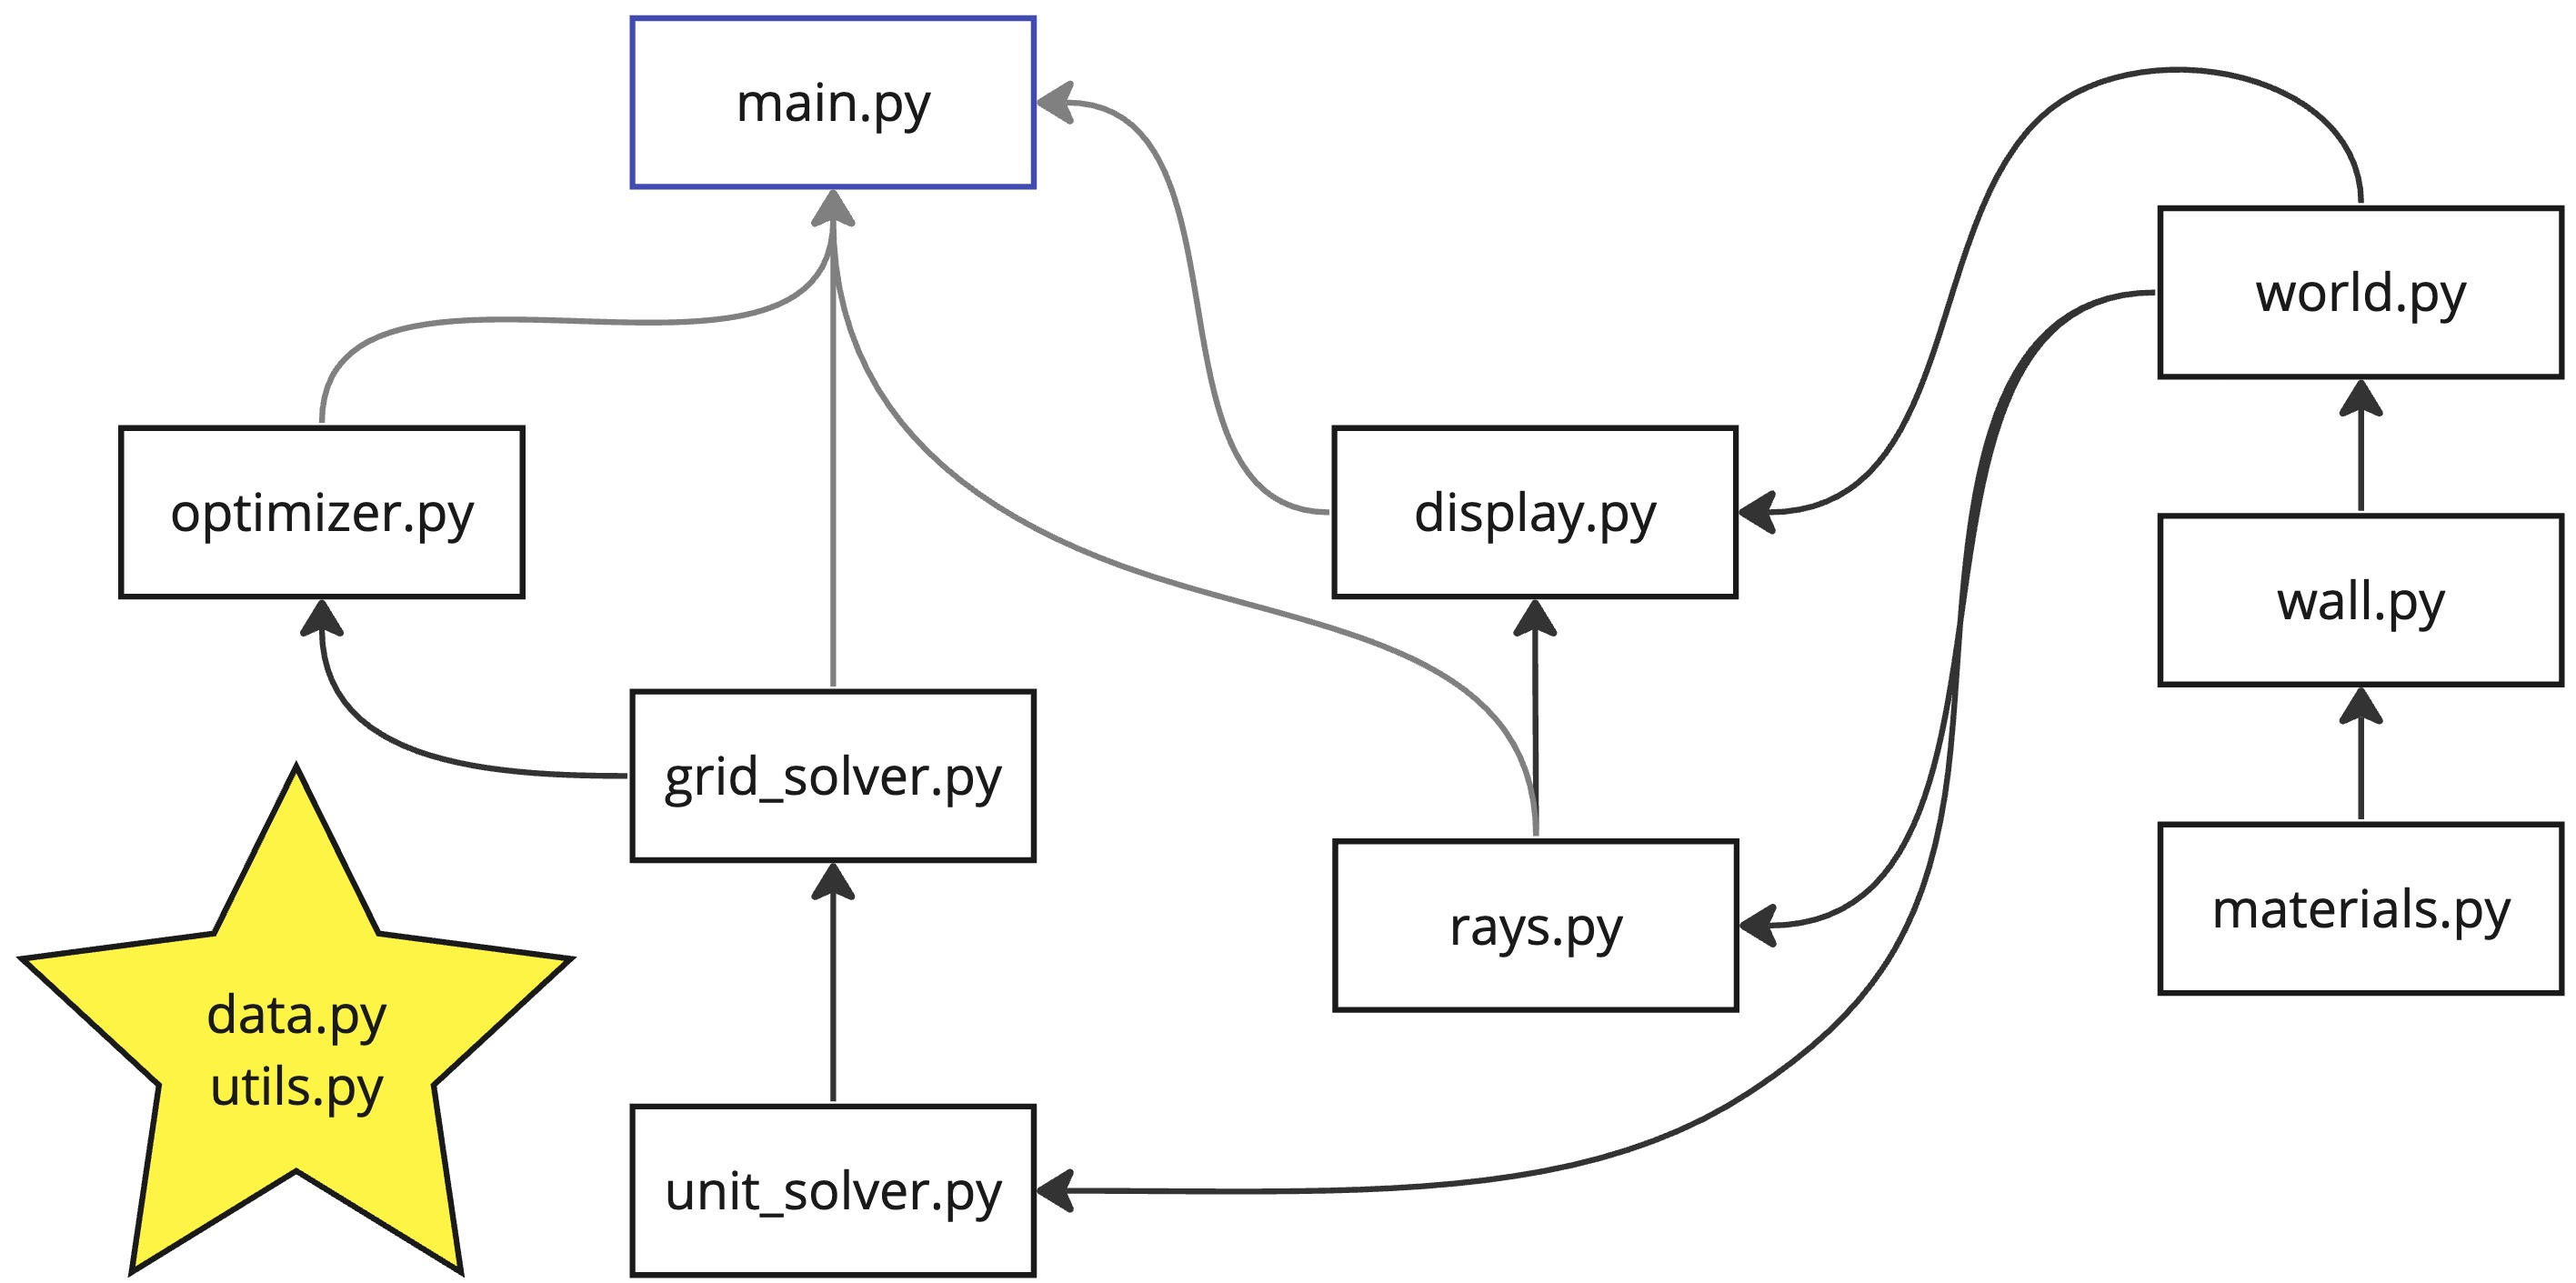
\includegraphics[width=0.6\textwidth]{images/programme.jpeg}
\end{figure}

\subsection{World}

L'objet \textbf{world} contient tous les \textbf{wall} d'abord en mémoire dynamique provisoire
puis transférée dans le gpu.

Chaque objet \textbf{wall} contient ses coordonnées, ses vecteurs unitaires $\vec{u}$ (tangent)
et $\vec{n}$ (normal) et une instance du \textbf{material} le décrivant.
Cet objet \textbf{material} contient les propriétés $\epsilon_r, \gamma$ et pré-calcule $Z, \gamma$.

La classe \textbf{Wall} contient des méthodes \texttt{@static} pour calculer les coefficients
de réflexion $\Gamma$ et transmission $T$ en module carré.

\subsubsection{Optimisation: AoS vs SoA}
une fois le transfert dans le gpu achevé, 
\textbf{world} va contenir ses \textbf{wall} sous forme 
d'\texttt{arrays} et non sous forme d'objets
par exemple les normales de tous les murs seront dans une grande array.
Un mur sera juste un indice dans ces grandes \texttt{arrays}.

Si on arrange mal notre mémoire on peut augmenter le taux de \textit{cache miss}

Par exemple, si on demande la normale au mur 3, il est fort probable
que l'on demande aussi son vecteur tangent, ses coordonnées, etc. 
Il serait pratique d'avoir ses informations stockées proches 
les unes des autres.
C'est pourquoi nous utilisons un stockage \texttt{AoS : array of structures}
plutôt que \texttt{SoA : structure of arrays}
\begin{lstlisting}[language=python,title=https://docs.taichi-lang.org/docs/layout]
# address: low ...................... high
# AoS:     RGBRGBRGBRGBRGBRGB.............
# SoA:     RRRRR...RGGGGGGG...GBBBBBBB...B    
\end{lstlisting}

On accompli cela dans le code au moment d'allouer la mémoire dans 
des \texttt{dense fields} de taichi
\begin{lstlisting}{language=python}
    ti.root.dense(ti.i, self.m).place(self.r0, self.r1, self.u, self.n, self.l, self.gamma, self.Z, self.eps_r)
    # instead of 
    # ti.root.dense(ti.i, self.m).place(self.r0)
    # ti.root.dense(ti.i, self.m).place(self.r1)
    # and ...
    # which would give us a SoA
\end{lstlisting}

Bien que beaucoup de murs partagent leur matériaux en communs,
ceux-ci ont été dupliqués. Cela a rendu le code plus simple (car accès à toutes les propriétés du mur par un indice) 
et à peut être aussi rendu l'accès mémoire plus localisé mais ça n'a
pas été vérifié.


\subsubsection{Optimisation sur le calcul des angles}

Passer par les fonctions trigonométriques $\arccos$ puis $\cos$ et $\sin$
est lent pour l'ordinateur.

\textbf{Wall} ne calcule donc pas les angles mais plutôt les fonctions trigonométriques
directement comme montré dans l'exemple \ref{subsub:2rebond}.

\subsection{Unit Solver}

Le fichier \textbf{unit\_solver} contient les méthodes pour calculer la puissance moyenne qu'on
obtiendra en un point $rx$ depuis un point $tx$ en calculant chaque réflexion et transmission de tous les rayons possibles.

\subsubsection{Transmission}

Une fonction \texttt{find\_intersection(r0, u, p2, q2)} pour trouver l'intersection entre
un mur et un rayon en renvoyant un paramètre $t$ qui donne le point par $\vec{r} = t \vec{u}$.
\warningsign ce paramètre ne garanti pas encore que l'on a une intersection physique.
Pour cela, il faut passer à la fonction suivante: \texttt{intersect(u, n, p1, q1, p2, q2)}
(avec p1, q1 les points extrêmes du mur et q2, p2 le rayon). Ici on vérifie d'abord que p2 et q2 soient chacun d'un côté different du mur grace
a leur produit scalaire avec $\vec{n}$, 
puis on regarde le point d'intersection ip et on determine par $sign(<ip-p1,u>) ?= sign(<ip-q1,u>)$ 
si il fait partie du mur ou non. 

On peut maintenant définir \texttt{wall\_transmission(world, p2, q2, index1=-1, index2=-1)}
qui va prendre un rayon et itérer parmi tous les murs voir avec la fonction
\texttt{intersect} si il faut calculer un coefficient de transmission (par la fonction dans \textbf{Wall}) dans
quel cas il sera multiplié au coefficient global de transmission renvoyé par la fonction.
Si l'on sait que le rayon part d'un mur ou rebondit sur un mur, \texttt{index1,2} permet 
de les enlever de la boucle.

\subsubsection{Reflexion}
Avant de traiter les réflexions, on prévoit la fonction \texttt{bounce\_cond(r0, n, tx, rx)}
pour verifier l'existence physique de cette dernière par rapport au mur avec
$sign(<n,p2 - r0>) ?= sign(<n,q2 - r0>)$ ($r0$ un point du mur et $p2,q2$ le rayon)


\subsubsection{Mise en commun}
On arrive à la fonction principale \texttt{calculate\_power(world, tx, rx)} dont
le but va être de remplir la fonction \eqref{f:p_moy}.

\begin{enumerate}
    \item[0] Elle calcule d'abord la
composante directe avec \texttt{wall\_transmission} et la distance entre $tx$ et $rx$
    \item[1] Puis on passe au premier itérateur des murs: au sein de celle-ci,
on utilise le tracé géométrique pour obtenir le trajet, on vérifie si la réflexion
est physique avec \texttt{bounce\_cond}, on trouve le point d'intersection avec
\texttt{find\_intersection},
on vérifie par une méthode analogue à celle dans \texttt{intersect} si ce point fait partie du mur.
Et enfin on calcule les coefficient de transmission de chaque rayon avec \texttt{wall\_transmission}
et les coefficient de réflexion pour chaque rayon avec là méthode statique \texttt{Wall.get\_rn2} (module carré).
    \item[2] On place dans ce premier itérateur le deuxième pour traiter des réflexions doubles.
On vérifie d'abord qu'on ne fait pas une réflexion double sur le même mur.
Ensuite, le tracé géométrique demandant d'abord le calcul du dernier (deuxième) point d'intersection,
on procède aux mêmes verification et calculs en marche arrière jusqu'à retomber sur $tx$
puis de calculer les coefficients pour chaque rayon.
\end{enumerate}


\begin{tcolorbox}[colback=red!10!white,colframe=red!50!black,title=Remarque,sharp corners]
    L'execution d'un code dans le gpu rend la definition d'un algorithme récursif inutile.
    Étant donné que la recursion n'est pas disponible, 
    pour une fonction de recursion qui se rappelle n fois, le compilateur
    devrait générer et compiler une fonction non recursive pour chaque changement de n.
    Le nombre de réflexions étant seulement de 2, il n'est pas grave d'expliciter le tout en 2 for-loops.
\end{tcolorbox}

\subsection{Grid}

La classe Grid parallelise \texttt{calculate\_power} de \textbf{unit\_solver} sur une grille 3D de $rx$ pour $n$ émetteurs.
La puissance moyenne est donc calculée pour tous ces points, on sélectionne
ensuite la puissance maximale parmi les $n$ émetteurs. Ceci fait, on peut convertir
le tout en $dbm$ et en débit binaire.

\subsubsection{Conversion en débit binaire}

On a une relation linéaire de la puissance en $dbm$ vers le débit binaire en $\log$

On construit donc une fonction pour passer de l'un à l'autre qui devrai
 être utilisée que dans le gamme (-90dbm à -40dbm)

\begin{table}[H]
\centering
\begin{tabular}{|ccc|}
    \hline Sensibilité & Débit binaire & log(Débit binaire) \\
    \hline$-90 \mathrm{dBm}$ & $50 \mathrm{Mb} / \mathrm{s}$ & 6 + log(50) \\
    \hline$-40 \mathrm{dBm}$ & $40 \mathrm{~Gb} / \mathrm{s}$ & 9 + log(40) \\
    \hline
\end{tabular}
\end{table}

\begin{align*}
    &f \colon x \in [-90, -40] \longrightarrow 6 + \log(50) + \frac{3 + \log(40) - \log(50)}{50} (x + 90)\\
    &\text{débit binaire} = 10^{f(x)}
\end{align*}

\subsubsection{Optimisation par la librairie Taichi}
La librairie python \texttt{taichi} permet d'une part de compiler des fonction
python en languages plus rapide et d'autre part de paralléliser
les for-loop au scope d'execution le plus haut dans les fonction ayant le décorateur
\texttt{@ti.kernel}. La compilation et l'execution en parallèle dans le cpu permet
déjà d'atteindre l'ordre de $10^{-2}s$ puis avec le passage au gpu : $10^{-3}s$ pour une grille
de cellules $10cm\times10cm$ sur le plan de OPERA-WCG.

Ici on compte aussi le temps pour pouvoir utiliser les données en dehors du contexte de taichi
sans quoi il semblerait que l'on puisse descendre encore un peu sur le
temps d'execution pour l'option gpu (l'option cpu ne souffrant pas vraiment de ces transferts de données).
L'idéal aurait alors été de centrer la conception du programme autour de l'algorithme d'optimisation
pour éviter ces transfers gpu-cpu.

\subsubsection{Optimisation: pourquoi paralléliser sur la grille de rx ?}
Une autre option aurait été de paralléliser le calcul sur la double for-loop de \texttt{calculate\_power} directement.
Seulement, on cherche à paralléliser le plus d'elements possible et si on compare:
\begin{itemize}
    \item 17 murs, double for-loop : $\rightarrow 17^2 = 289$
    \item grille de $0.5m$ minimum, calcul en tout point de la grille : $\rightarrow \frac{8}{0.5} \times \frac{15}{0.5} = 480$
\end{itemize}

Il est donc preferable de paralléliser sur la grille.





\subsection{Data \& Utils}
data.py \& utils.py sont partagés par tous les fichiers, 
ils contiennent d'une part toutes les données pour
caractériser le problème et d'autre part des import et méthodes souvent utilisés

Les données introduite dans le logiciel pour OPERA-WCG et pour le problème illustratif
du syllabus d'exercice sont dans l'annexe \ref{sub:data}

\subsection{Affichage}
\textbf{display} s'occupe de plot les données. Il peut faire appel à \textbf{Rays}
qui contient tous les rayons à (0,1,2) rebonds pour un couple $(tx,rx)$ donné.

L'objet \textbf{display} fera aussi appel à \textbf{world} pour qu'il utilise \textbf{display}
pour dessiner les murs avec le code couleur suivant:
\begin{table}[H]
    \centering
    
\begin{tabular}{|c|c|c|c|} 
    \toprule
    Matériaux & $\epsilon_r$ & $\sigma$ & couleur \\
    \midrule
    % Brique & 3,95 & 0,073 & \textcolor{}{} \\
    % \midrule
    Béton & 6,4954 & 1,43 & \textcolor{red}{$\blacksquare$}\\
    \midrule
    Cloison & 2,7 & 0,05346 & \textcolor{green}{$\blacksquare$}\\
    \midrule
    Vitre & 6,3919 & 0,00107 & \textcolor{cyan}{$\blacksquare$}\\
    \midrule
    Paroi métallique  & 1 & $10^7$ & \textcolor{gray}{$\blacksquare$} \\
    \bottomrule
\end{tabular}

\end{table}





\section{Verification}

\subsection{Exercice du syllabus}
\begin{figure}[H]
    \centering
    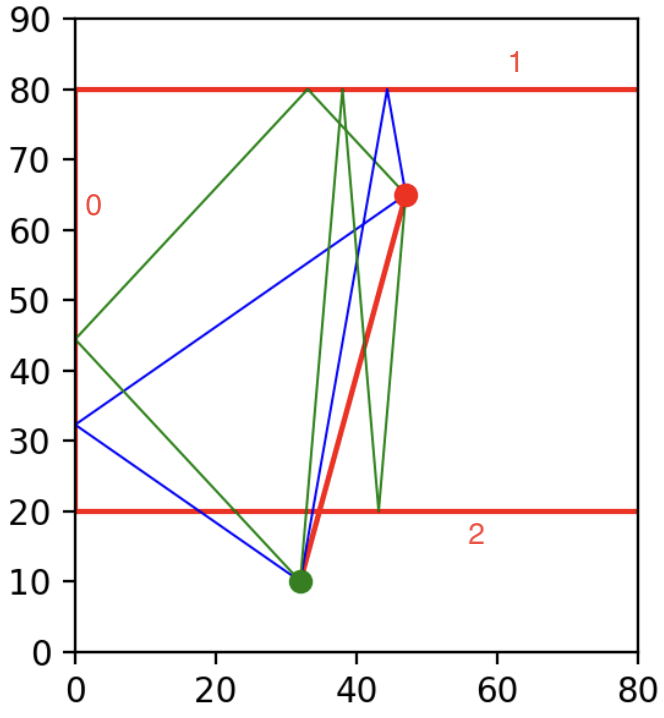
\includegraphics[width=0.35\textwidth]{images/verif/rayons.png}
    \caption{Sortie du programme quand on entre les données de l'exercice. les axes sont en [m]. Les murs sont nommés de 0 à 2}
    \label{f:ray_ex}
\end{figure}

\begin{figure}[H]
\begin{lstlisting}[language=python]
direct : Prx 3.336E-10 <-
first bounce : wall 0 : Prx 1.039E-11 <-
second bounce : wall 0,1 : Prx 4.136E-12 <-
first bounce : wall 1 : Prx 9.554E-12
second bounce : wall 1,2 : Prx 1.287E-13
total rays: 5
\end{lstlisting}
\caption{stdout du programme quand on entre les données de l'exercice}
\end{figure}

On utilise ici la classe \textbf{Rays} pour le calcul, car celle ci
possède une fonction \texttt{calculate\_power} modifiée pour stocker les
points de rayons et afficher les puissance partielles (pour chaque composante à (0,1 ou 2) réflexions)

Les paramètres pour ce problème sont en commentaire dans l'annexe \ref{sub:data}.
\subsubsection{Calcul pour un exemple à deux rebonds}
\label{subsub:2rebond}

Les formules importantes ont été écrites dans \textit{mathematica} pour faciliter
le calcul avec les nombres complexes. 

\begin{figure}[H]
    \centering
    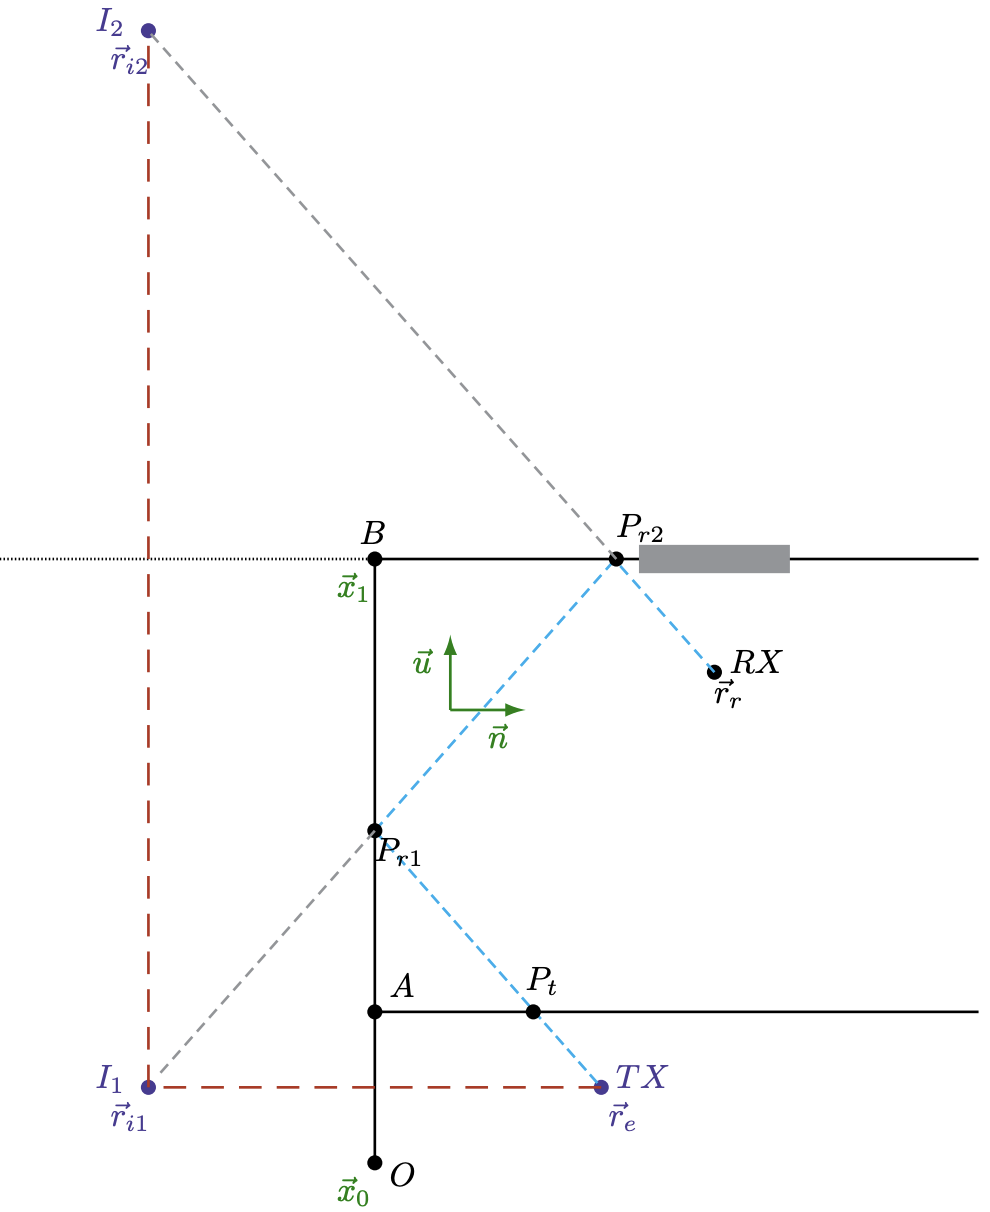
\includegraphics[width=0.4\textwidth]{images/verif/2_rebonds.png}
    \caption{Tracé géométrique du problème, $tx = (32, 10)$ et $rx = (47, 65)$}
    \label{f:exemple}
\end{figure}

On commence par trouver géométriquement les points $\vec{r}_{i1}, \vec{r}_{i2}$

\begin{align*}
    &\vec{r}_{i1} = (-32, 10) &\vec{r}_{i2} = (-32, 150)
\end{align*}

On voit qu'on aura une transmission en $Pt$ et 2 réflexions en $Pr1, Pr2$

On doit trouver ces points d'intersection avec les murs.
Pour cela il suffit de faire une interpolation linéaire de 2 points du rayons
et de regarder le point $x$ ou $y$ pour lequel on intersecte le mur.
La connaissance de $Pt$ requiert la connaissance de $Pr1$ qui lui meme requiert $Pr2$.

Commençons donc par $Pr2$:
On fait une interpolation linéaire de $\vec{r}_{i2}$ à $\vec{r}_{r}$ $\equiv f(x)$

\begin{align*}
    &f(x) = y_{i2} + \frac{y_r - y_{i2}}{x_r - x_{i2}}(x - x_{i2})
    = 150 - \frac{85}{79}(x + 32)\\
    &\textrm{on cherche $x$ pour avoir $y=f(x)=y_{mur1}=80$}\\
    &f(x) = 80 \iff x = 33.05 = x_{Pr2}
\end{align*}

Finalement : $Pr2 = (33.05, 80)$

On peut effectuer des calculs presque identiques et obtenir $Pr1 = (0, 44.435)$ et $Pt = (22.707, 20)$

Il ne reste qu'à calculer les angles d'incidence $\cos(\theta_i), \sin(\theta_i)$ 
et de transmission $\cos(\theta_t), \sin(\theta_t)$
avant de pouvoir calculer les coefficient de transmission et de réflexions.

Commençons par les angles de la transmission sur le mur 2 (voir figure \ref{f:ray_ex})

\begin{equation}
\label{f:cos_i}
    \begin{aligned}
    & \cos \theta_i=\left|<\frac{\vec{d}}{\|d\|}, \vec{u}>\right|=\frac{d_y}{\|d\|}=0.732532
    \end{aligned}
\end{equation}
Dans cette formule \eqref{f:cos_i}, on a pris $\vec{u}$ pour avoir
le vecteur normal à la surface du mur et on a définit un vecteur
d'incidence $\vec{d} = Pr1 - \vec{r}_e$

$\sin(\theta_i)$ est obtenu simplement par $\sqrt{1 - \cos(\theta_i)^2} = 0.680733$

Ensuite l'angle de la transmission dans le mur est donné par $\sin(\theta_t) = \frac{\sin(\theta_i)}{\sqrt{\epsilon_r}} = 0.31071$
et $\cos(\theta_t) = \sqrt{1 - \sin(\theta_t)^2} = 0.950505$

Le coefficient de réflexion de surface pour une polarisation perpendiculaire

\begin{equation}
    \Gamma_{\perp}\left(\theta_i\right)=\frac{Z_m \cos \theta_i-Z_0 \cos \theta_t}{Z_m \cos \theta_i+Z_0 \cos \theta_t} = -0.48052 + 0.014901j 
\end{equation}

On définit $s = \frac{l}{cos(\theta_t)} = 0.157811$ la distance parcourue dans le mur.

\begin{equation}
    T_m\left(\theta_i\right)=\frac{\left(1-\Gamma_{\perp}^2\left(\theta_i\right)\right) e^{-\gamma_m s}}{1-\Gamma_{\perp}^2\left(\theta_i\right) e^{-2 \gamma_m s} e^{j \beta 2 s \sin \theta_t \sin \theta_i}}=
    0.62948 + 0.0890456j
\end{equation}

On calcule de manière similaire les paramètres pour les 2 réflexion en utilisant
\begin{equation}
    \Gamma_{m}\left(\theta_i\right)=\Gamma_{\perp}\left(\theta_i\right)-\left(1-\Gamma_{\perp}^2\left(\theta_i\right)\right) \frac{\Gamma_{\perp}\left(\theta_i\right) e^{-2 \gamma_m s} e^{j \beta 2 s \sin \theta_t \sin \theta_i}}{1-\Gamma_{\perp}^2\left(\theta_i\right) e^{-2 \gamma_m s} e^{j \beta 2 s \sin \theta_t \sin \theta_i}}
\end{equation}
\begin{align}
    &\Gamma_{m,1} = -0.471151 + 0.251816j 
    &\Gamma_{m,2} = -0.419027 + 0.246183j
\end{align}

On voit géométriquement (figure \ref{f:exemple}) que la distance est $|\vec{r}_r - \vec{r}_{i2}|$ et en utilisant la formule \eqref{f:p_moy}:

\begin{align}
    <P_{RX}> = P_{RX0} \times |T_{m}|^2 \times |\Gamma_{m,1}|^2 \times |\Gamma_{m,2}|^2 \frac{1}{d^2} = 4.127 \times 10^{-12}
\end{align}

\subsubsection{Verification avec le code}

Dans le syllabus, vu que l'on calcule les champs, on obtient des phénomènes 
d'interference non present dans la puissance moyenne. Il faut donc
faire attention a bien prendre les résultat qui utilisent la puissance moyenne.

\begin{table}[htbp]
    \centering
    \caption{Verification puissances moyennes [W]}
    \label{tab:my_table}
    \begin{tabular}{c|c|c}
        \toprule
        Murs & Puissance Syllabus ou Calculée & Puissance Code \\
        \midrule
        direct $\times$ & $3.33 \times 10^{-10}$ & $3.336 \times 10^{-10}$ \\
        une réflexion avec 0 & $1.039 \times 10^{-10}$ 
        \tablefootnote{Dans le sylla on a le resultat en $dBm$ de la puissance moyenne
            comptant la transmission directe et le premier rebond sur le mur 0.
            En passant en $W$ et en soustrayant la composante directe, on obtient bien
            le resultat affiché
        } & $1.039 \times 10^{-10}$ \\
        deux réflexions avec 0 puis 1 & $4.127 \times 10^{-12}$ & $ 4.136 \times 10^{-12} $\\

        % Fill in your data here
        \bottomrule
    \end{tabular}
\end{table}

\subsection{Verification du tracé de rayons}

On se place dans le cas un peu plus complexes des bureaux de OPERA-WCG.

\begin{figure}[H]
    \centering
    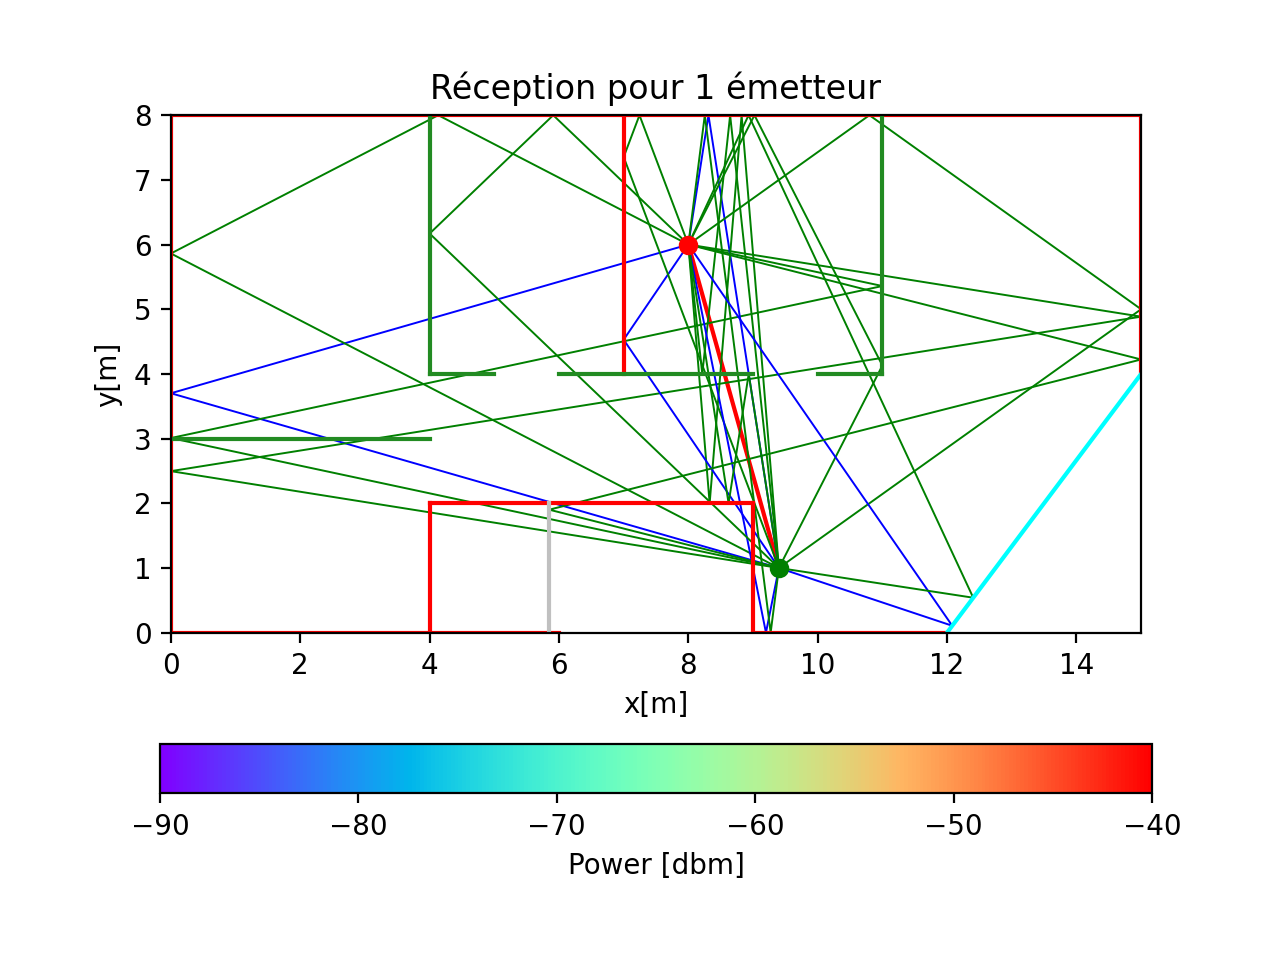
\includegraphics[width=0.5\textwidth]{images/verif/rayons_complex.png}
    \caption{tx = (9.4, 1.0), rx = (8.0, 6.0)}
\end{figure}

\begin{figure}[H]
    \centering
    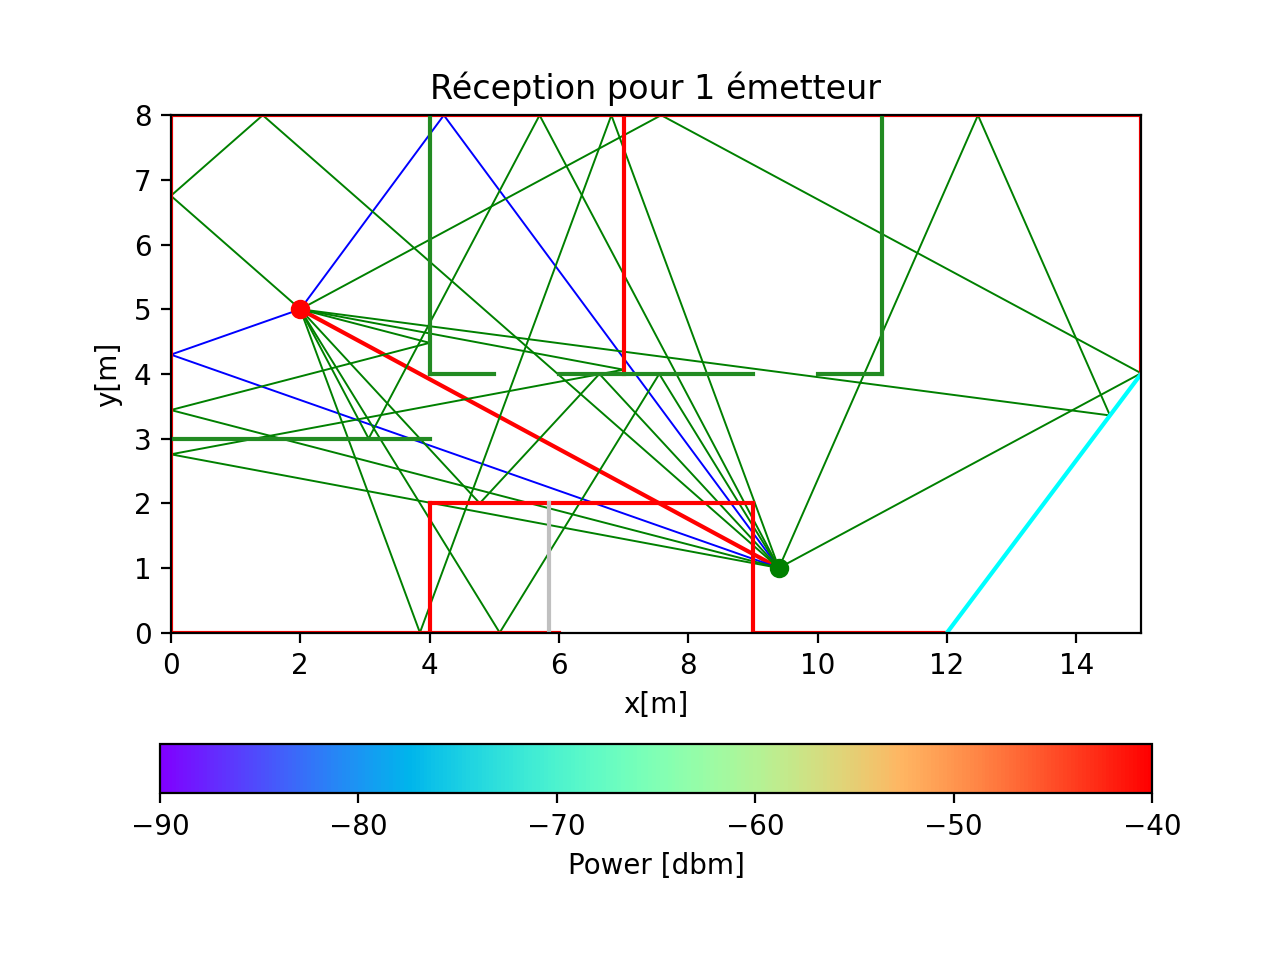
\includegraphics[width=0.5\textwidth]{images/verif/rayons_complex_2.png}
    \caption{tx = (9.4, 1.0), rx = (2.0, 5.0)}
\end{figure}

Tous les rayons semblent être explicable par l'optique géométrique.
    

\section{Résultat de calcul}

\begin{figure}[H]
    \centering
    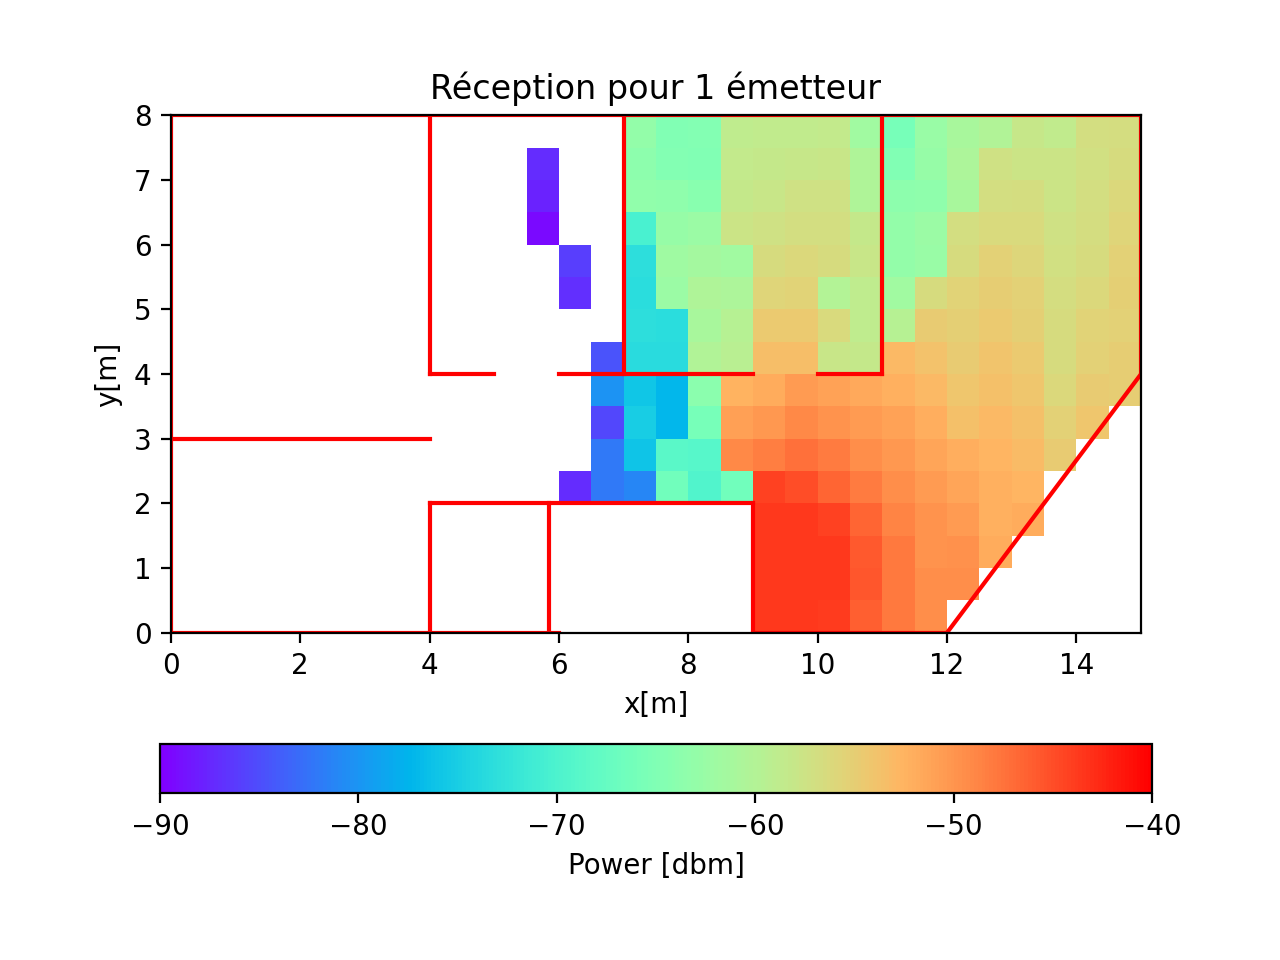
\includegraphics[width=0.49\textwidth]{images/base.png}
    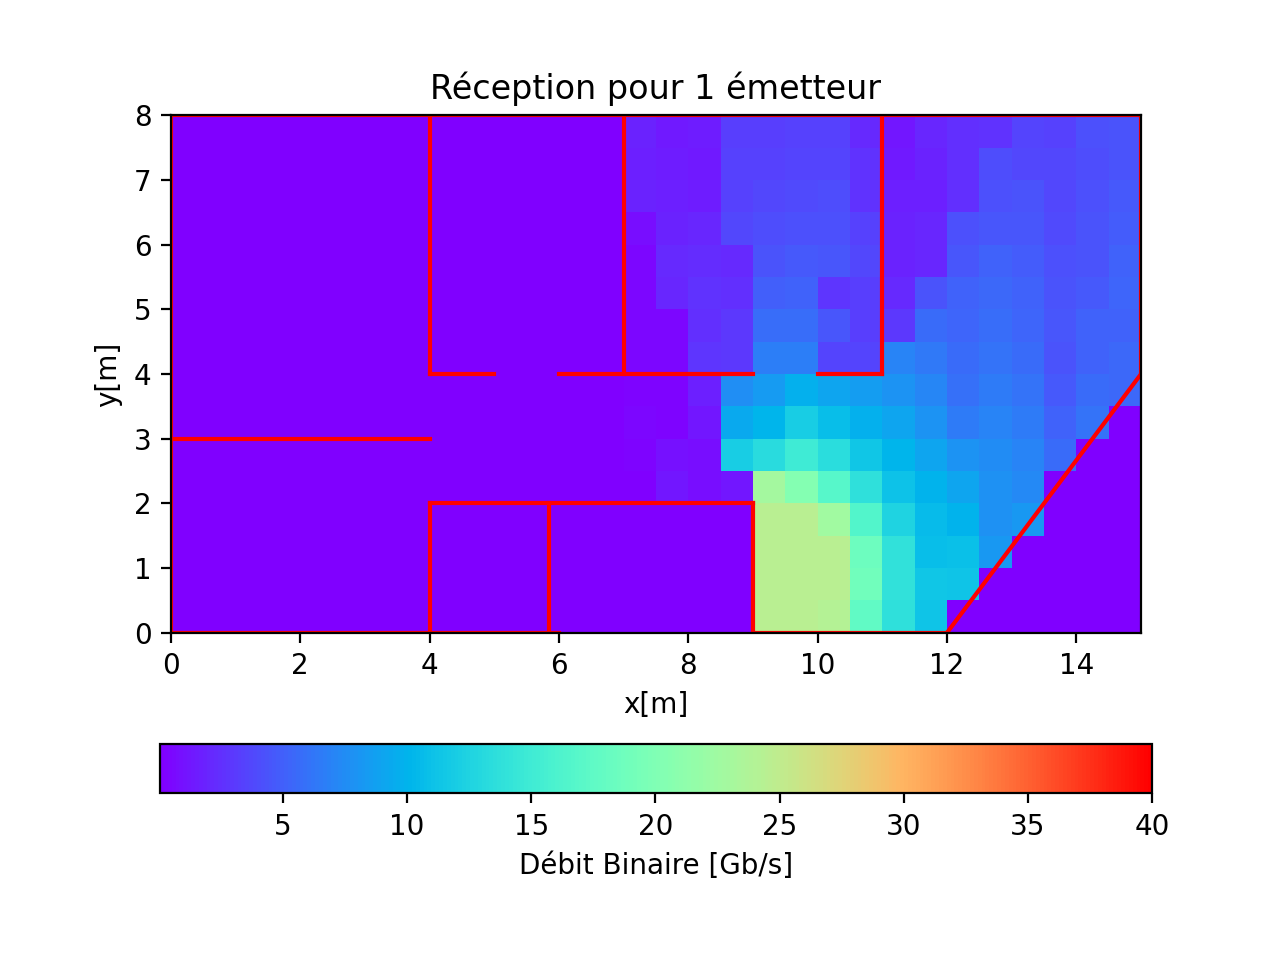
\includegraphics[width=0.49\textwidth]{images/base_binaire.png}
    \caption{Émetteur dans la position suggérée : tx = (9.4, 1.0)}
\end{figure}

La profondeur de peau de notre béton à cette fréquence : $\delta = \frac{1}{105.63} < 1cm$.
Les murs ayant une épaisseur de 30cm, il n'y aura jamais aucune onde qui passera au travers
pour atteindre l'ascenseur.
On supposera donc que l'ascenseur n'est pas là pour réduire le temps de calcul. 

On constate aussi qu'un unique émetteur dans la position suggérée ne suffira pas à couvrir l'ensemble des bureaux.

\section{Suggestion pour améliorer la reception}

Le but ici va être de trouver un compromis entre nombre d'émetteurs (donc prix) et couverture.

\subsection{Recherche de maximum}
Pour commencer, il faut savoir où placer ces émetteurs. pour cela,
nous allons utiliser un algorithme de recherche de maximum global.
Nous sommes ici en presence d'un problème peu continu car changer un peu 
la position d'un émetteur
peu d'un coup le permettre atteindre une nouvelle piece.
Dans ce cadre peu continu, les algorithmes conventionnels purement déterministes
auront du mal à converger.

C'est pourquoi il a été nécessaire de prendre un algorithme avec une partie un peu
plus aléatoire, "brute force", d'evolution générationnelle. Celle-ci à été mélangée
avec un algorithme de manipulation géométrique pour l'étape de mutation. Cet algorithme
est appelé \textbf{évolution différentielle}.

% \begin{tcolorbox}[colback=blue!10!white,colframe=blue!50!black,title=Evolution differentielle,sharp corners]
%     L'evolution différentielle mélange algorithme génétique et technique géométrique.
%     Nous avons une population d'individus dont les mutations et recombinaisons sont dictées 
%     par une manipulation géométrique.
% \end{tcolorbox}

Nous prenons l'implementation de la librairie \textit{scipy}

\texttt{scipy.optimize.differential\_evolution(func, bounds, args=(n), strategy='best1bin', popsize=40)}
\begin{itemize}
    \item \textbf{func} sera notre fonction coût (voir plus loin)
    \item \textbf{bounds} délimite la zone dans laquelle on peut placer nos émetteurs (ici : l'appartement) 
    \item \textbf{pop\_size} augmentera la population d'essais ce qui augmentera nos chances de tomber sur le maximum global.

\end{itemize}

\subsection{Architecture d'optimisation}

Le plus important ici est de trouver une fonction coût pour emmener l'algorithme
vers la solution de manière rapide et fiable.
Ici nous prenons $f = \sqrt{\sum_{i,j}power[i,j]^2}$ que l'algorithme tentera de maximiser.
Prendre le carré des valeurs de puissance permet de punir d'avantage les endroits où
la reception est mauvaise et d'augmenter le gradient des valeurs de $f$ ce qui 
augmente la vitesse de convergence. 

Pour focaliser l'algorithme sur la maximisation de la couverture,
on ignore les valeurs de puissance au dessus de $-50dbm$ qui ne représente que la puissance
à immédiate proximité de l'antenne.

L'optimisation s'effectue sur une grille de pas $0.2m$. Les coordonnée optimales
trouvées sont ensuite affichée avec une grille de pas $0.05m$

L'algorithme a eu tendance à placer l'antenne pile dans un mur, ce qui empêchait la détection
de la transmission et donc de l'attenuation en résultant. Il a donc fallu ajouter une condition
pour éviter cet endroit.

\subsection{Essais d'optimisation}

Essayons avec un émetteur

\begin{figure}[H]
    \centering
    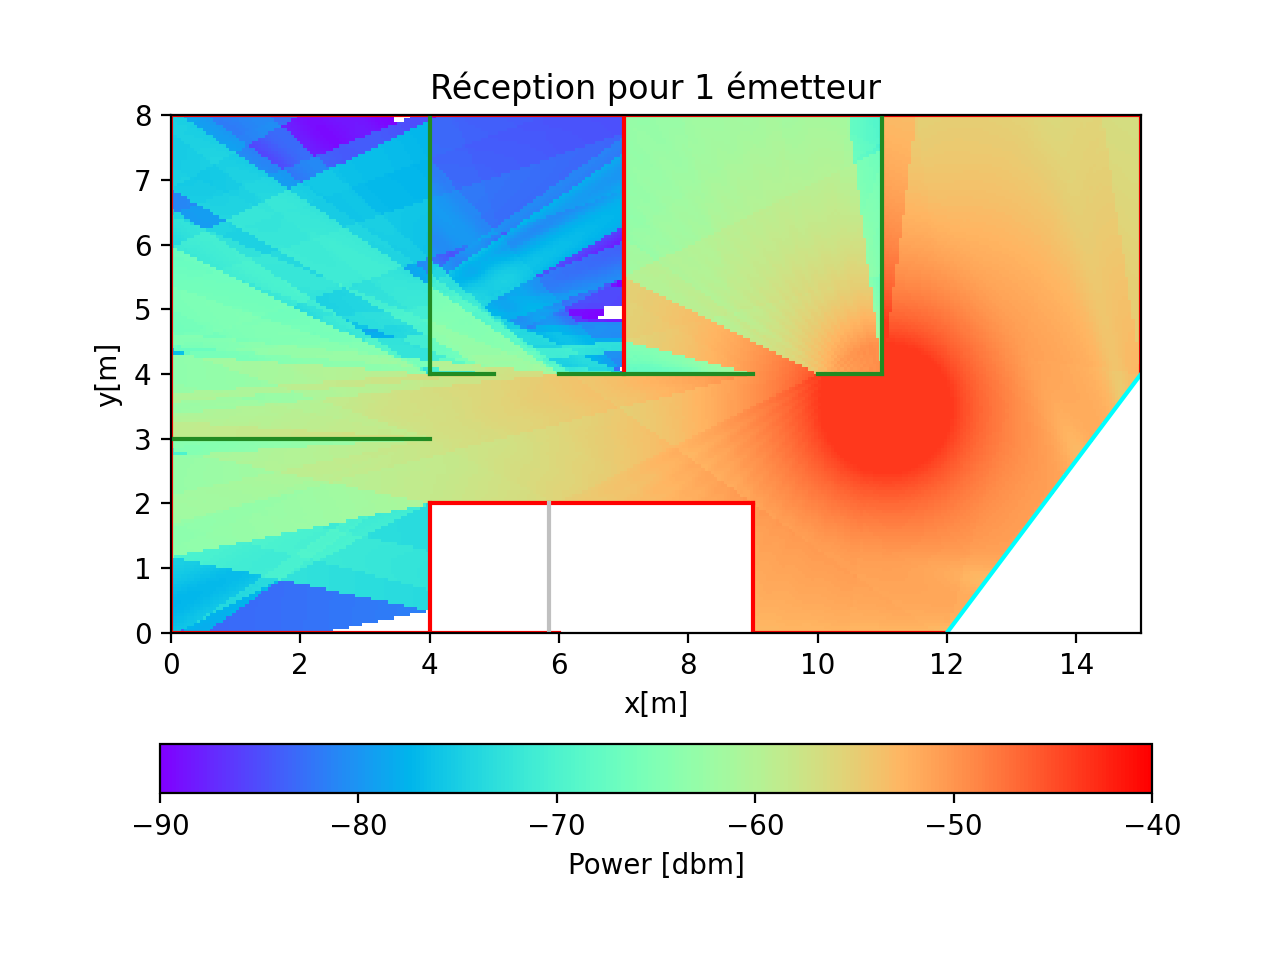
\includegraphics[width=0.49\textwidth]{images/opti/1.png}
    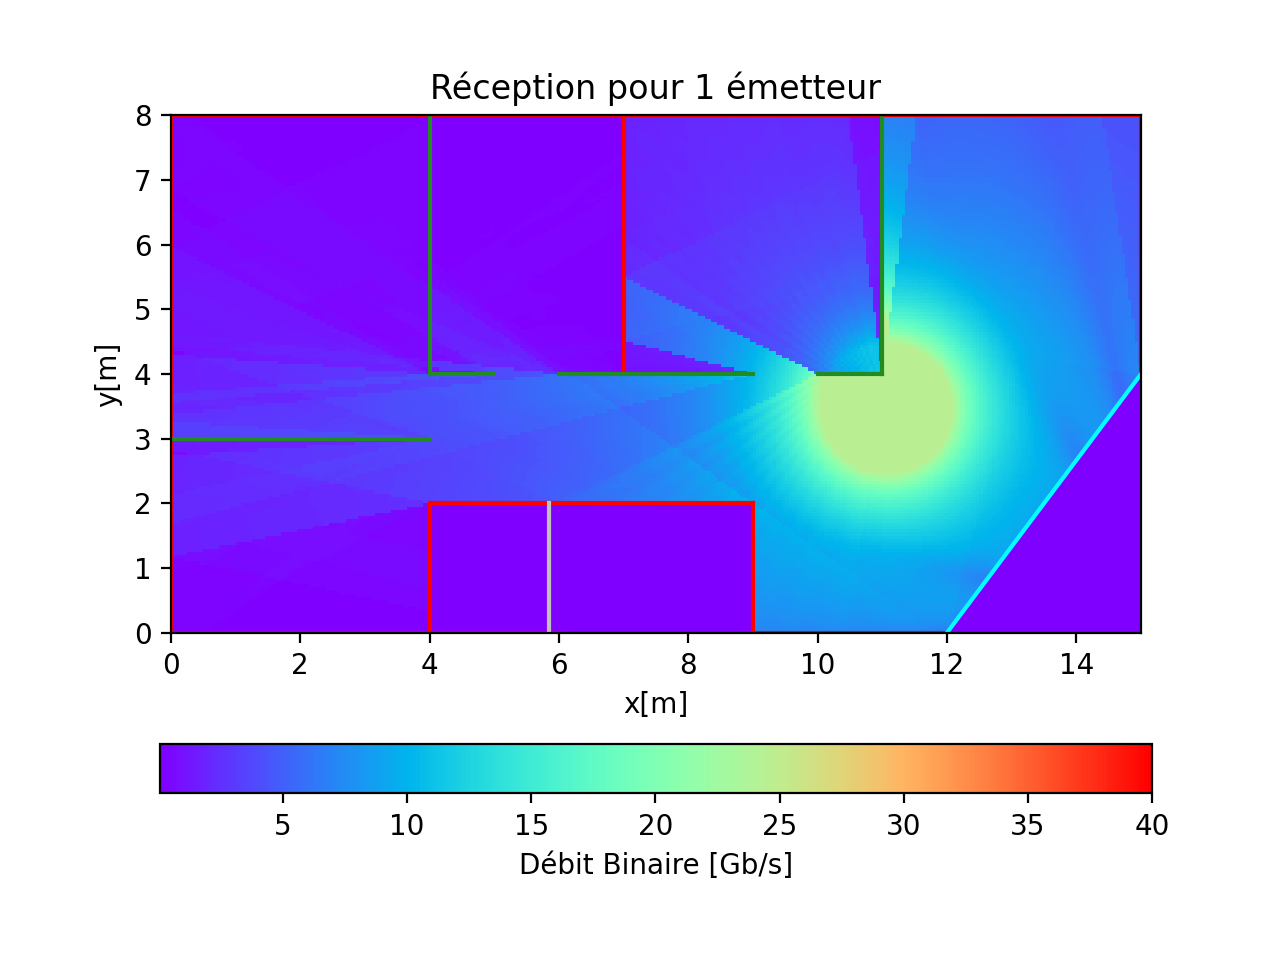
\includegraphics[width=0.49\textwidth]{images/opti/1_bin.png}
\end{figure}

On voit que c'est un peu mieux mais que ça reste insuffisant pour
couvrir l'ensemble de l'espace. On essaye donc avec 2 émetteurs.

\begin{figure}[H]
    \centering
    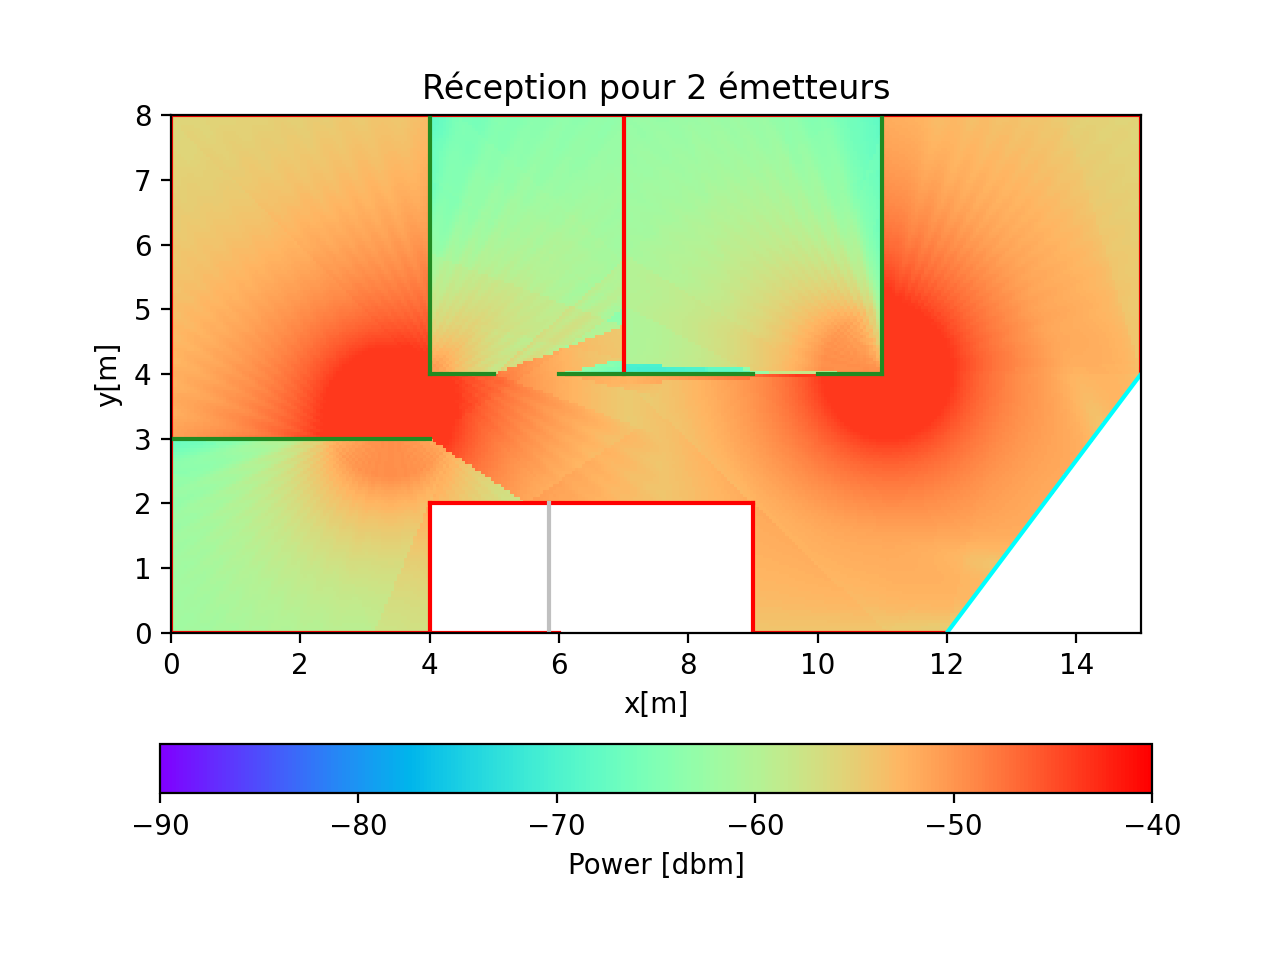
\includegraphics[width=0.49\textwidth]{images/opti/2.png}
    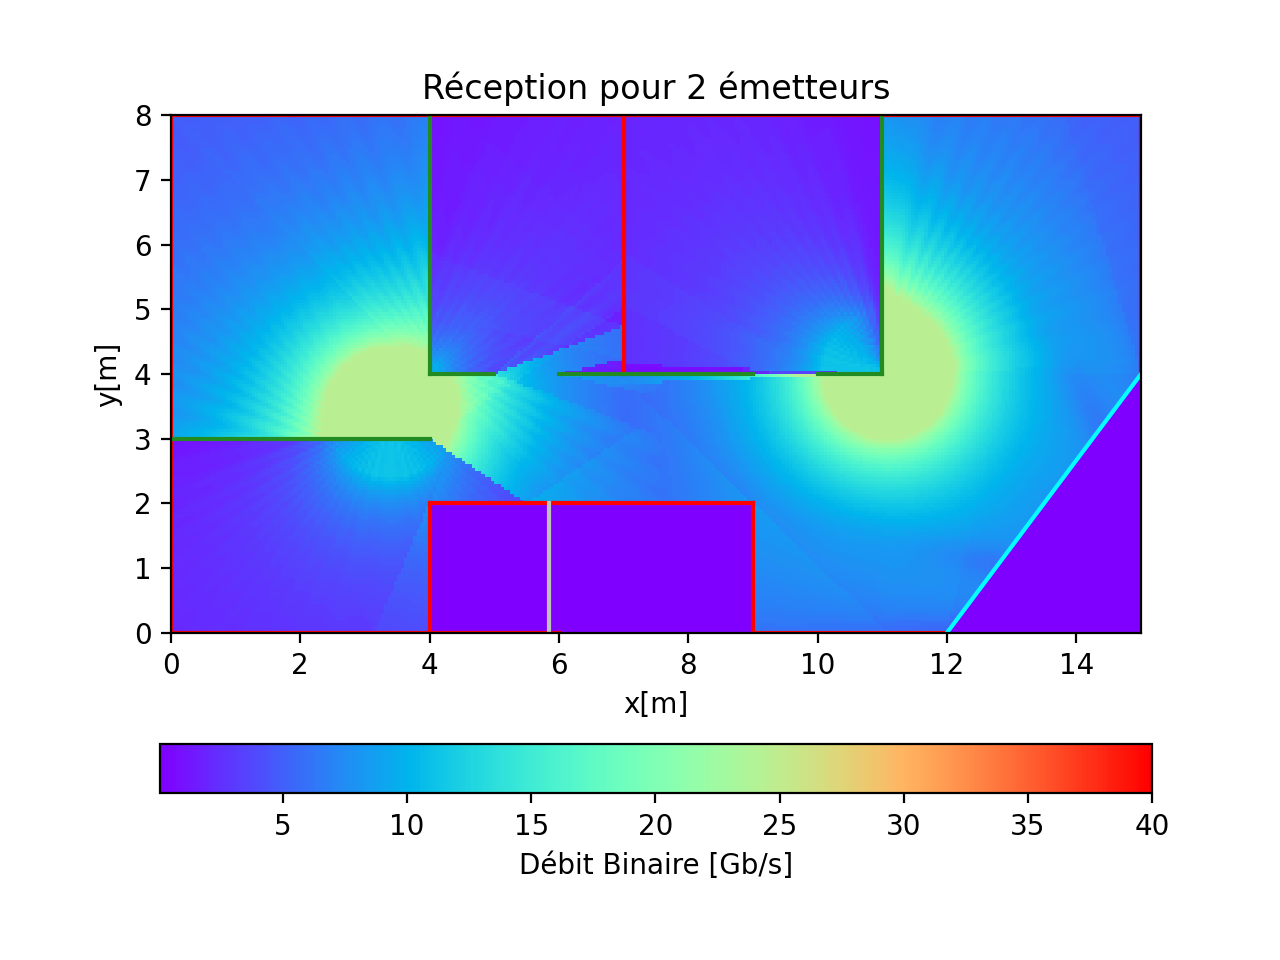
\includegraphics[width=0.49\textwidth]{images/opti/2_bin.png}
\end{figure}

On parviens à rester $\ge -65db$ partout ce qui équivaut à $1.4 Gb/s$.

Pour 3 émetteurs, il est difficile de trouver une solution unique
pour l'optimisation. Des exemples sont dans l'annexe \ref{sub-3}, leur fonction coût
ne varie que d'$1\%$. Les cas à 4,5 émetteurs sont aussi en annexes 
mais seront discutés plus tard.

\subsection{Combien faut-t-il d’émetteurs ?}
Plutôt que de montrer à chaque fois la répartition, regardons des variables
plus globales.

\begin{figure}[H]
    \centering
    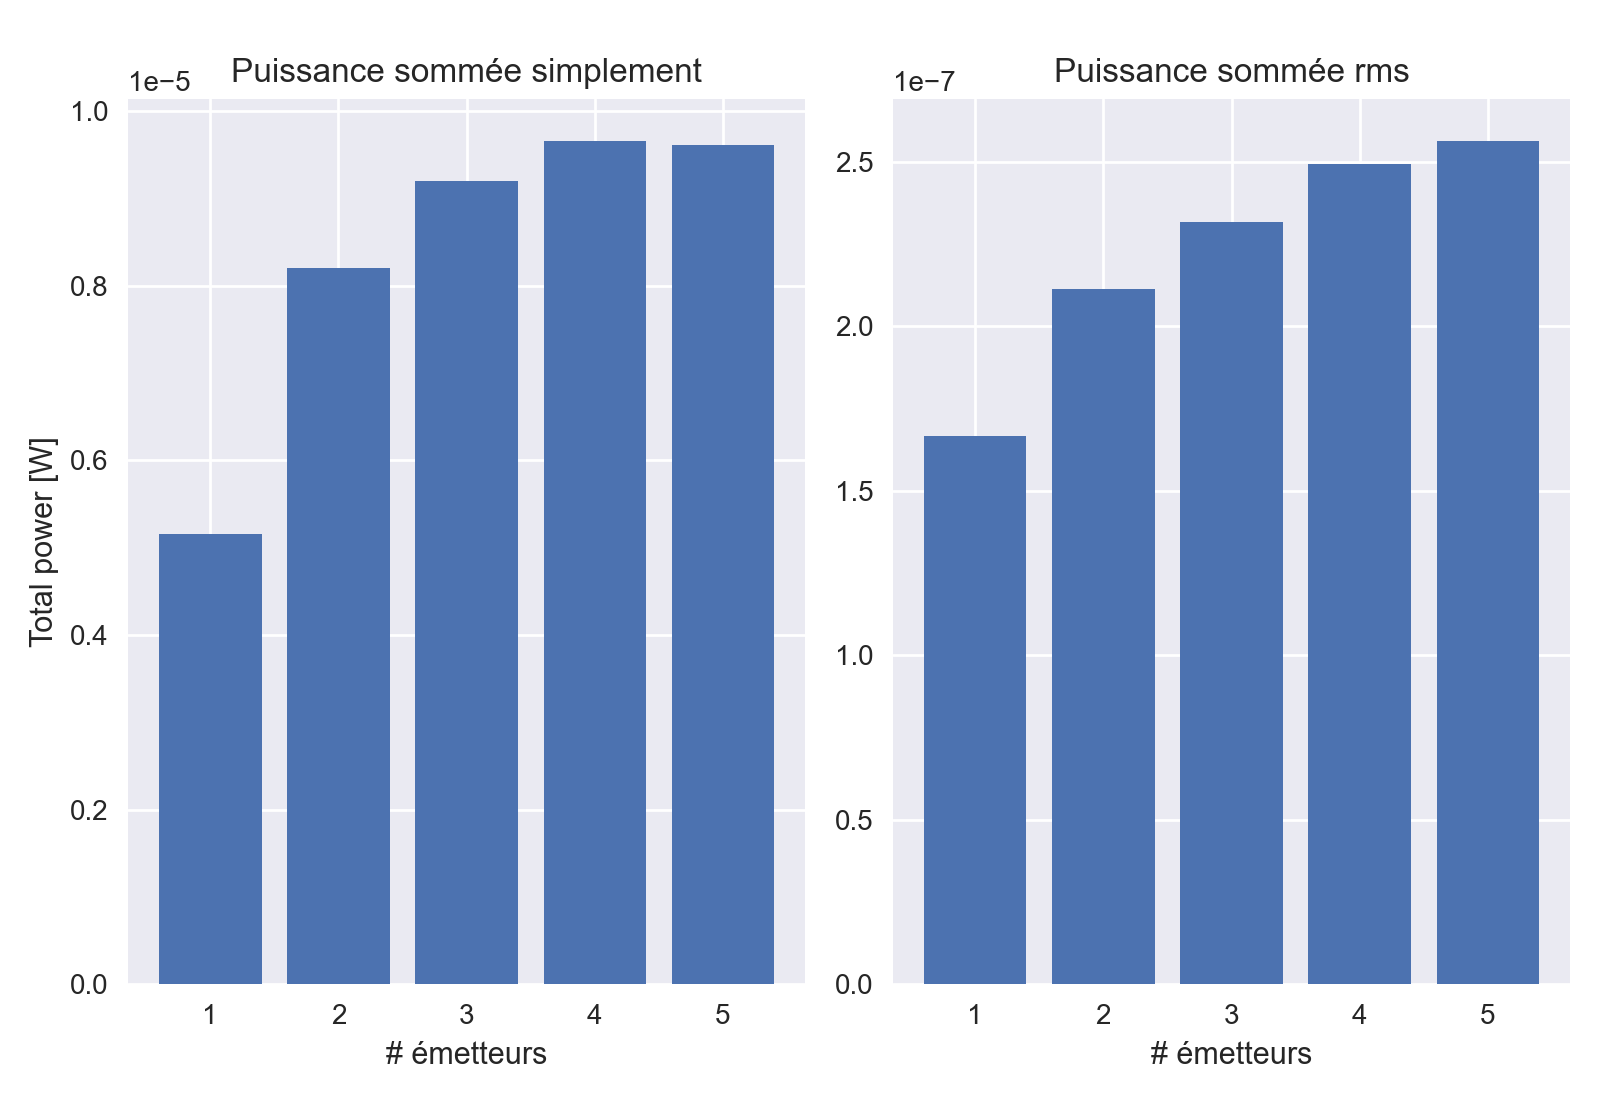
\includegraphics[width=0.8\textwidth]{images/opti/data_compare.png}
    \caption{Evolution de la couverture}
    \label{fig:datacomp}
\end{figure}

Attention, ici les fonctions coût sont différente. A gauche,
la fonction coût est une simple sommation des puissances, à droite,
on a la fonction coût comme décrite avant en \textit{rms}.

A partir de 5 émetteurs, le temps de calcul devient vraiment long,
pour une \texttt{pop\_size = 40} l'algorithme fait appel $212811$ fois à la 
fonction \texttt{get\_power()}

\begin{tcolorbox}[colback=blue!10!white,colframe=blue!50!black,title=Conclusion,sharp corners]
La figure \ref{fig:datacomp} montre que placer 2 émetteurs
est un minimum et qu'on atteint une presque saturation à partir de 4. 

Les figures de $3,4$ émetteurs (voir annexes \ref{sub-3}, \ref{sub-4}) montre que si 
on a le budget pour augmenter, il vaut mieux passer à 4 directement. 
3 émetteurs permettent d'augmenter la puissance globale (voir \ref{fig:datacomp})
mais pas encore d'atteindre une répartition homogène tandis que 4 émetteurs
permettent de s'en rapprocher suffisamment.
\end{tcolorbox}


\section{Annexes}

% \subsection{Données du problème du Syllabus}
% \begin{itemize}
%     \item $f = 868.3 \times 10^6$, $\omega = 2\pi f$, $\lambda = \frac{c}{f}$
%     \item $\beta = \omega \sqrt{\mu_0  \epsilon_0}$
%     \item $\epsilon_r = 4.8$
%     \item $\sigma = 0.018 S/m$
%     \item $l = 0.15m$
%     \item $Z_0 = 120\pi$
%     \item $R_{ar} = 73 \Omega$
%     \item $P_{tx} = 10^{-3} W$
% \end{itemize}

\subsection{Plus d’émetteurs}
\subsubsection{Trois émetteurs}
\label{sub-3}

\begin{figure}[H]
    \centering
    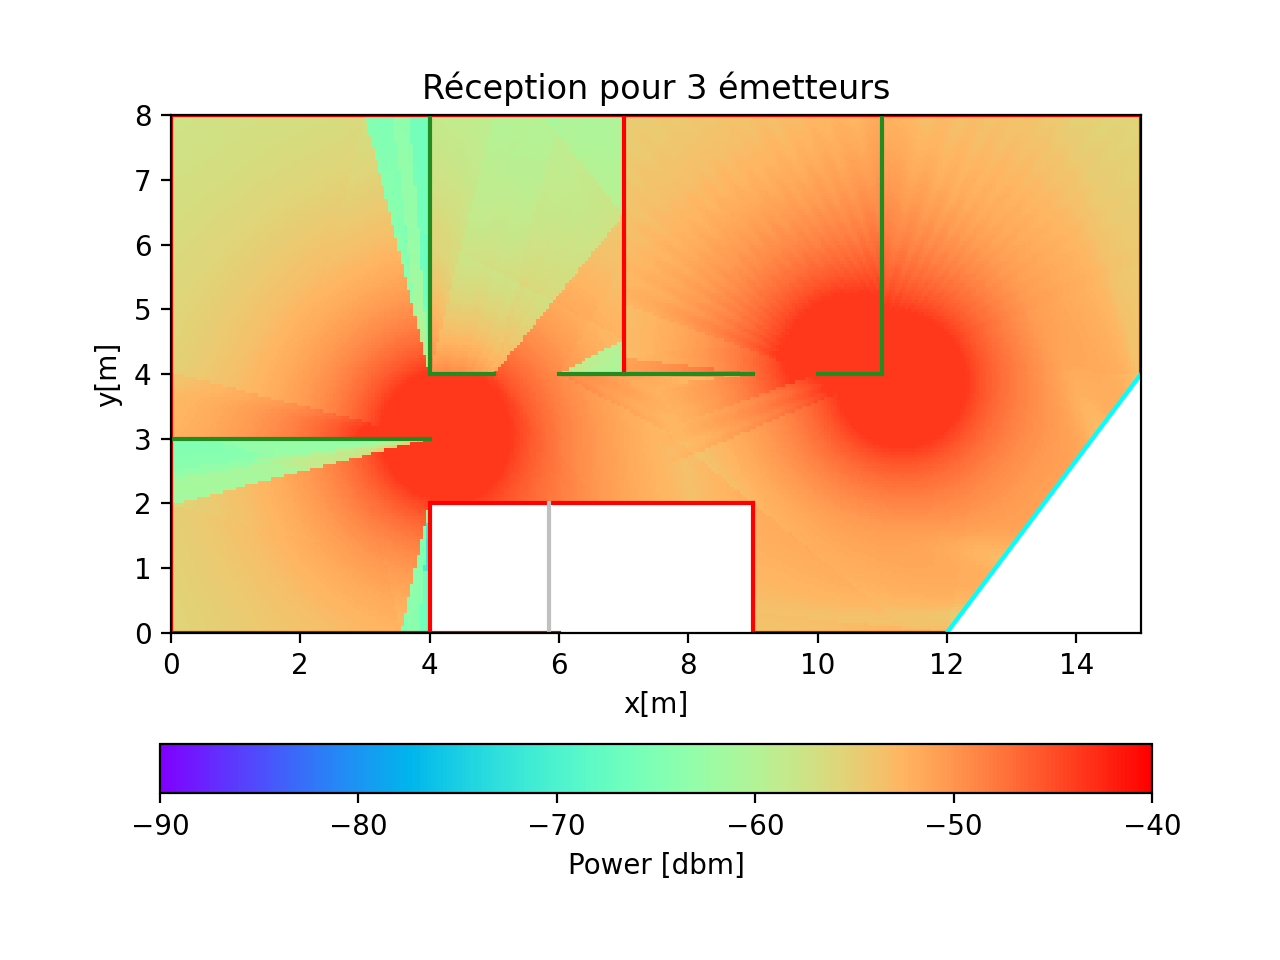
\includegraphics[width=0.49\textwidth]{images/opti/3.png}
    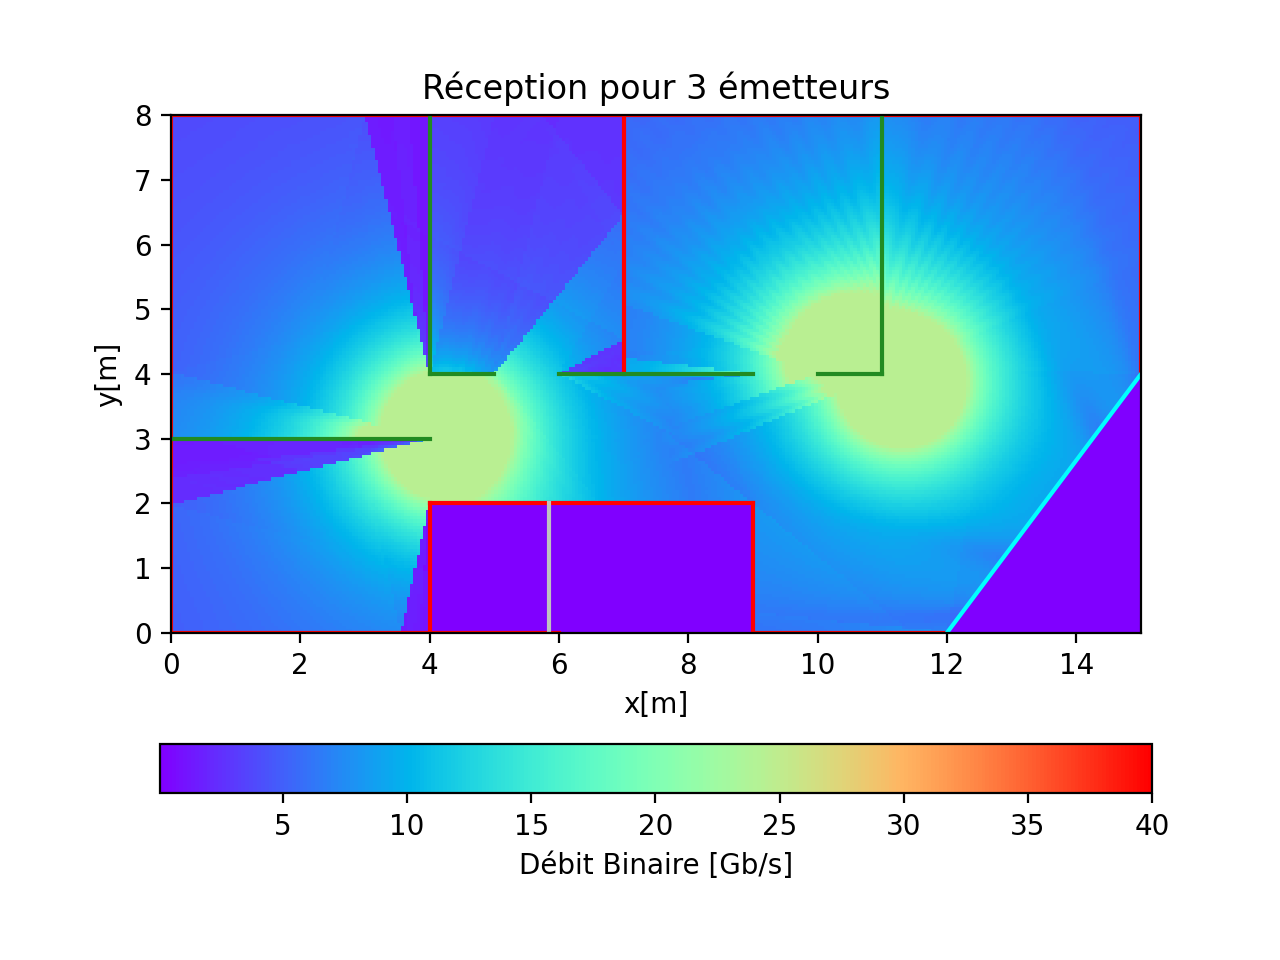
\includegraphics[width=0.49\textwidth]{images/opti/3_bin.png}
\end{figure}

\begin{figure}[H]
    \centering
    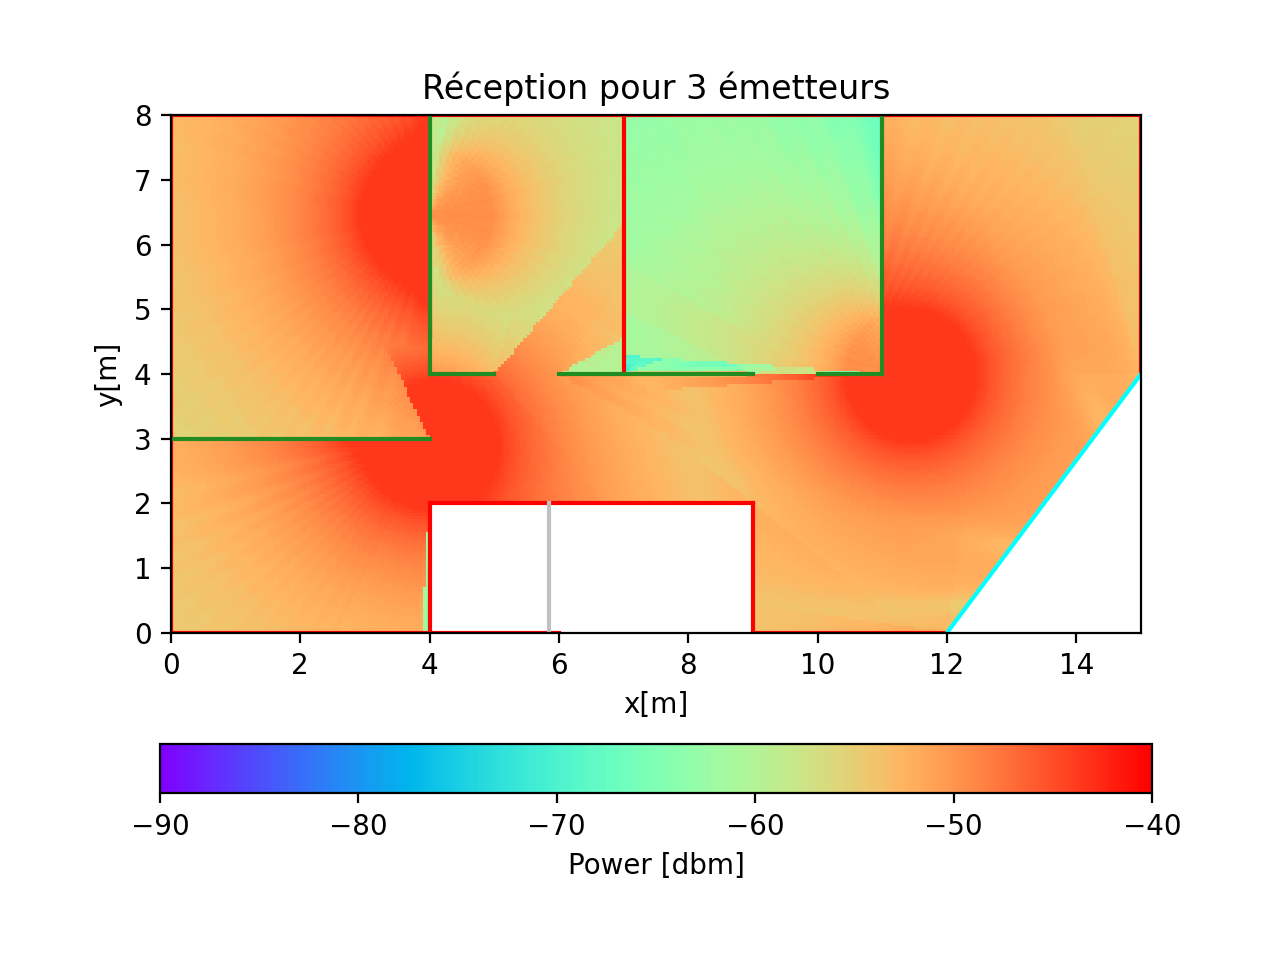
\includegraphics[width=0.49\textwidth]{images/opti/3_2.png}
    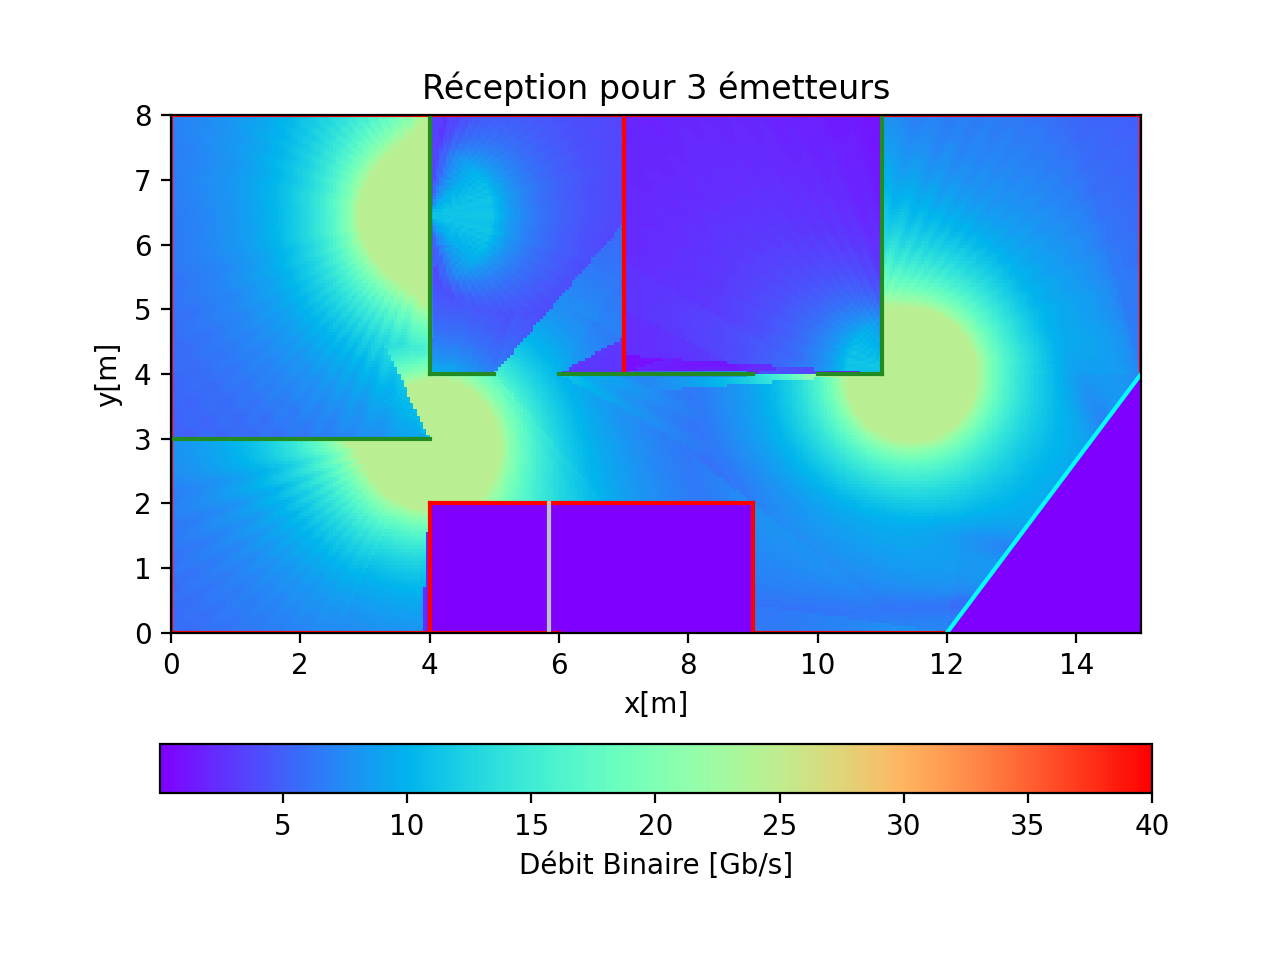
\includegraphics[width=0.49\textwidth]{images/opti/3_2_bin.png}
\end{figure}

\begin{figure}[H]
    \centering
    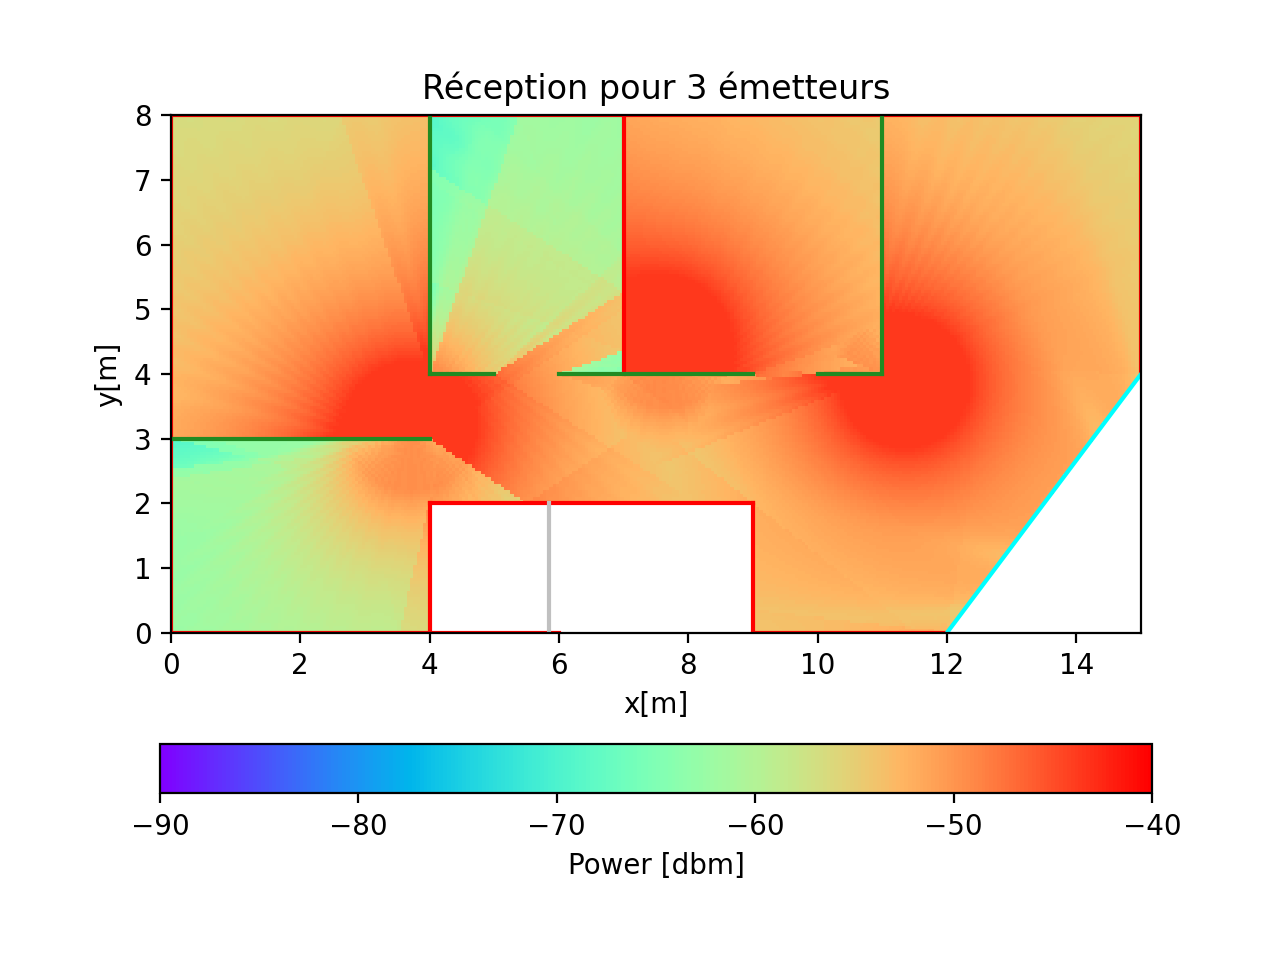
\includegraphics[width=0.49\textwidth]{images/opti/3_3.png}
    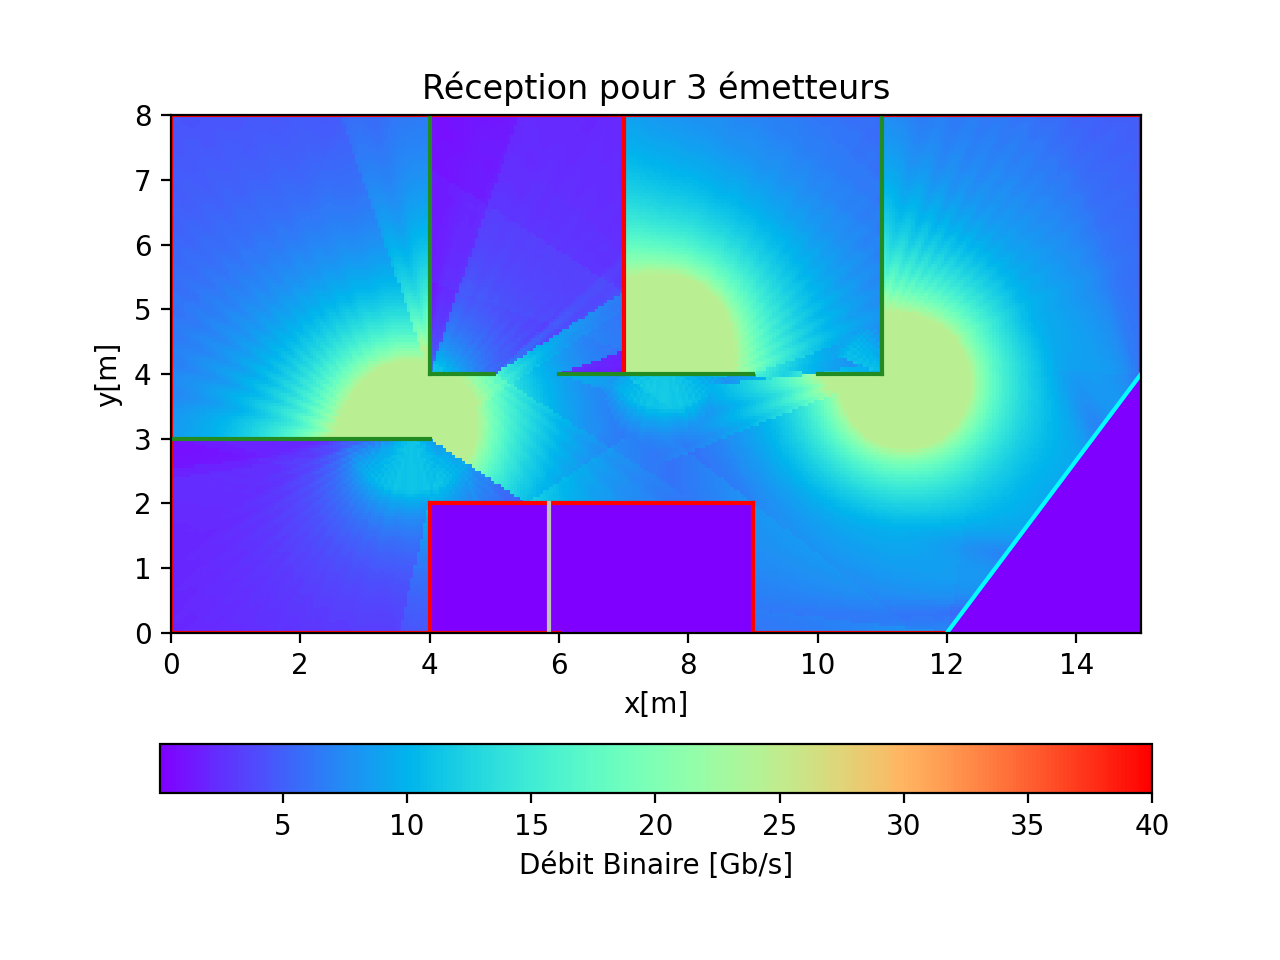
\includegraphics[width=0.49\textwidth]{images/opti/3_3_bin.png}
\end{figure}

\subsubsection{Quatre émetteurs}
\label{sub-4}

La solution à 4 émetteurs est stable car contrairement à la solution à
3 émetteurs, toutes les chambres peuvent être atteinte par des rayons direct
\begin{figure}[H]
    \centering
    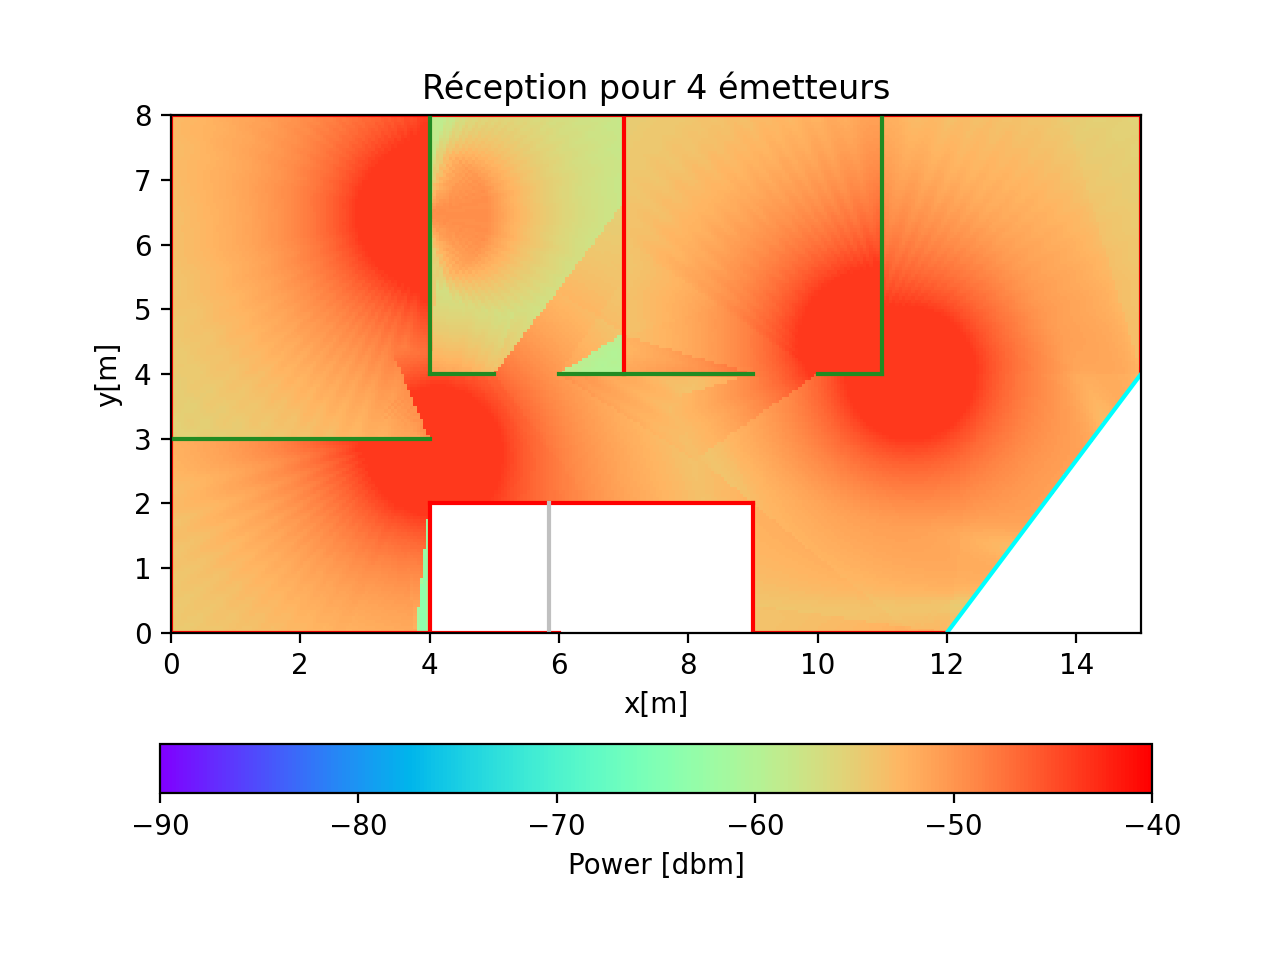
\includegraphics[width=0.49\textwidth]{images/opti/4.png}
    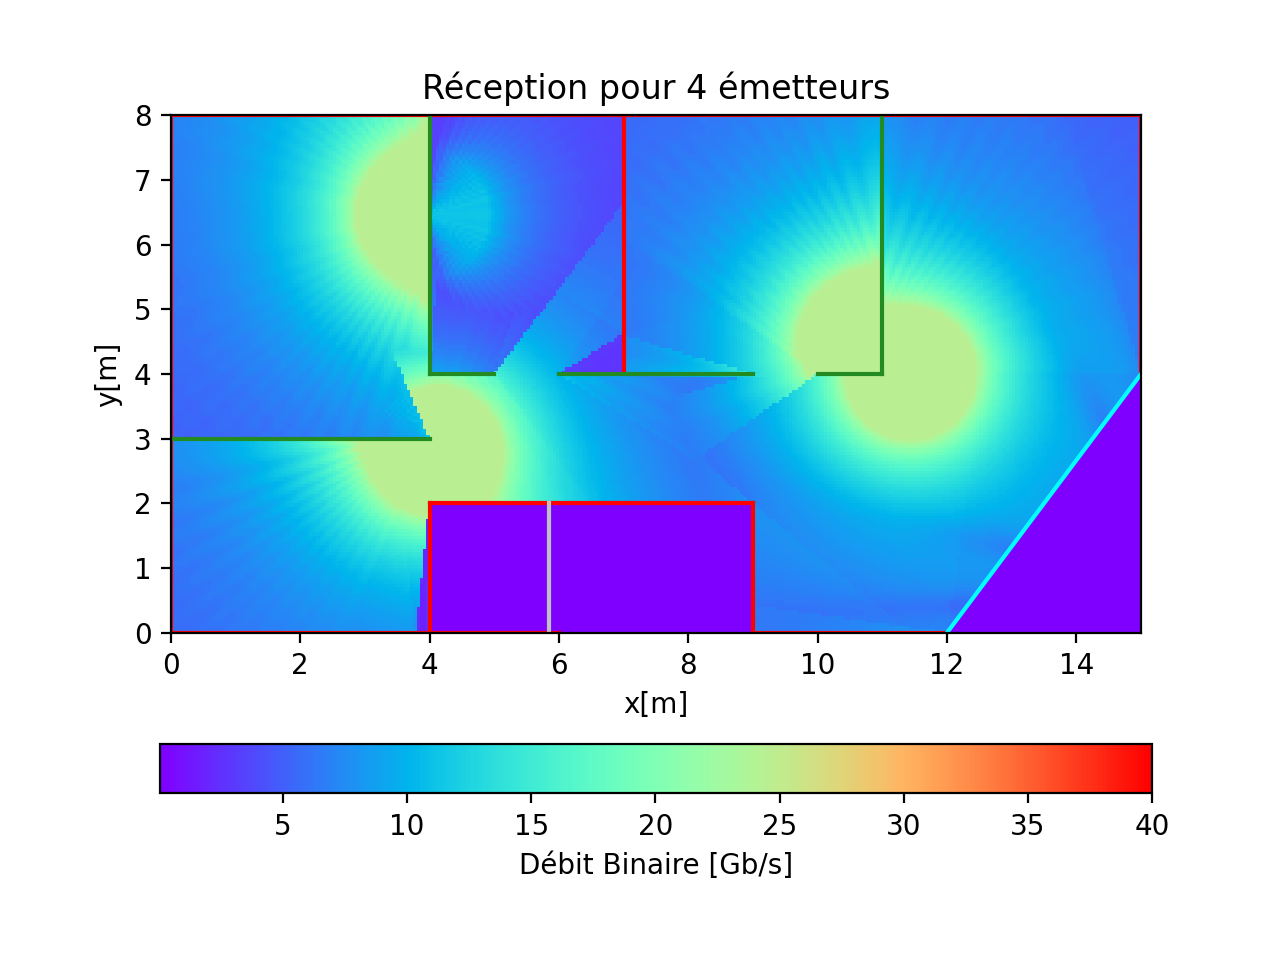
\includegraphics[width=0.49\textwidth]{images/opti/4_bin.png}
\end{figure}

\subsubsection{Cinq émetteurs}
\label{sub-5}

\begin{figure}[H]
    \centering
    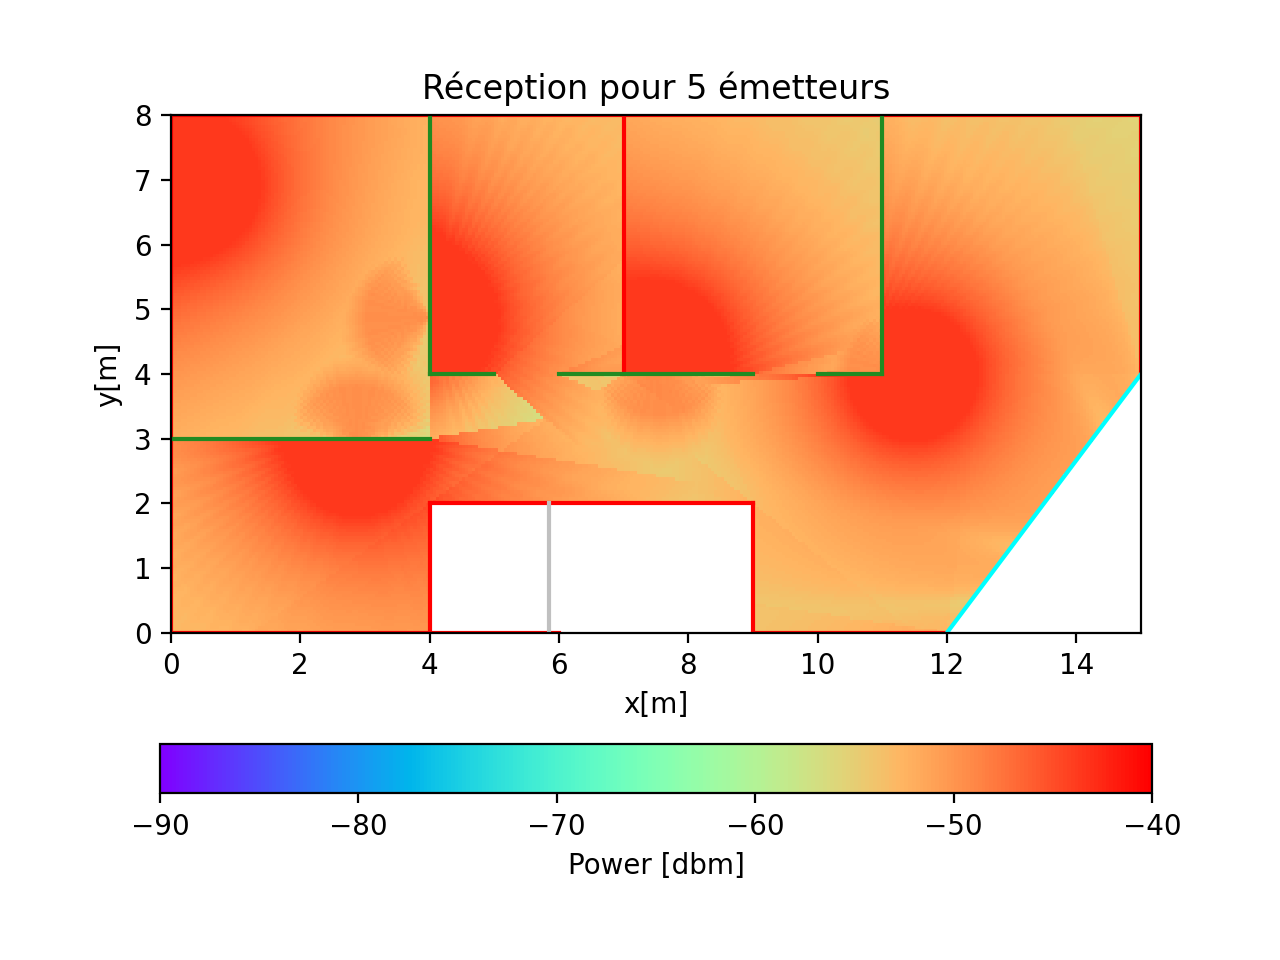
\includegraphics[width=0.49\textwidth]{images/opti/5.png}
    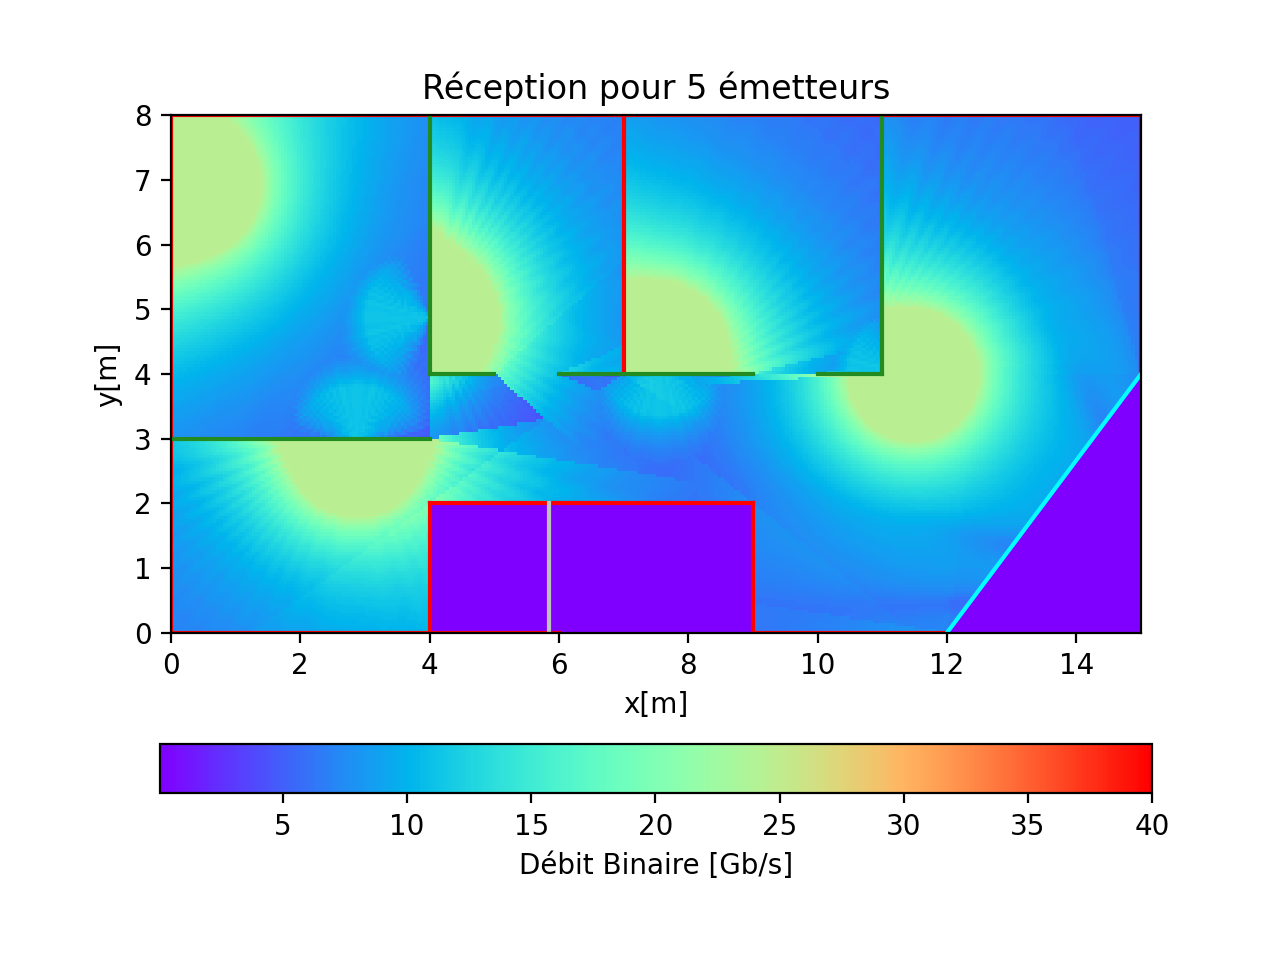
\includegraphics[width=0.49\textwidth]{images/opti/5_bin.png}
\end{figure}

La couverture est parfaite, 4 émetteurs étaient deja suffisant.


\subsection{Code}

\subsubsection{Main}

\begin{lstlisting}[language=python]
from world import world
from grid_solver import *
from display import image
from optimizer import *
from data import *
from rays import *

""" Allocating and transferring gpu memory for walls """
world.allocate()
world.transfer()

""" Optimisation """
grid = Grid(n)
grid.generate_grid()
result = txs_optimize(grid)
print(result)  # contains information like number of iteration, optimal position and cost function value
print("rms : ", grid.get_rms())
print("total : ", grid.get_total())

""" Use the optimized positions and
display it with a better resolution """
del grid  # freeing old data
dim.update(0.5)  # updating the resolution
precise_grid = Grid(n)
precise_grid.generate_grid()
txs = result.x.astype(np.float32)  # to use the optimized txs
# txs = tx.to_numpy()  # to use the tx defined in data
precise_grid.fill_power(txs)
precise_grid.power_to_dbm()  # fills array of dbm
precise_grid.dbm_to_binary()  # fills array of binary debit

""" Rays """
# rays.init_after_world(world, tx, rx)
# test_rays(rays)

""" Extract images """
image.re_init()
# image.draw_rays(rays)
image.plot_function(precise_grid.rx_powers_dbm.to_numpy(), "dbm")
image.plot_emitters(txs)
image.show()
image.extract(f"./exports/{n}_dbm.png")
image.re_init()
image.plot_function(precise_grid.rx_binary.to_numpy(), "binary")
image.plot_emitters(txs)
image.show()
image.extract(f"./exports/{n}_bin.png")

\end{lstlisting}

\subsubsection{Grid Solver}

\begin{lstlisting}[language=python]
from utils import *
from data import *
from unit_solver import calculate_power
from world import world


@ti.data_oriented
class Grid:
    def __init__(self, n):
        self.rx_centers = ti.Vector.field(2, dtype=ti.f32)
        self.rx_powers_n = ti.field(ti.f32)
        self.rx_powers = ti.field(ti.f32)  # where the best from rx_powers_n is extracted
        self.rx_powers_dbm = ti.field(ti.f32)  # converted to dbm
        self.rx_binary = ti.field(ti.f32)  # converted to binary debit
        self.n = n  # number of emitters
        ti.root.dense(ti.ijk, (dim.y, dim.x, n)).place(self.rx_powers_n)
        ti.root.dense(ti.ij, (dim.y, dim.x)).place(self.rx_centers)
        ti.root.dense(ti.ij, (dim.y, dim.x)).place(self.rx_powers, self.rx_powers_dbm, self.rx_binary)  # AoS

    @ti.kernel
    def generate_grid(self) -> ti.i32:
        # fills the rx_centers array with all rx coordinate with respect to cell size
        for i, j in self.rx_centers:
            x = dim.cell_size / 2.0 + j * dim.cell_size
            y = dim.cell_size / 2.0 + i * dim.cell_size
            self.rx_centers[i, j] = vec2([x, y])
        return 0

    @ti.kernel
    def fill_power(self, txs: ti.types.ndarray(dtype=ti.f32, ndim=1)):
        # accepting numpy array as pos makes the code slower here
        # but since the optimization algorithm sends numpy arrays of positions
        # this is still faster compared to manual conversion
        for i, j, k in self.rx_powers_n:
            # i,j are all the grid receiver points
            # k is the chosen emitter in the n sized array
            if self.rx_centers[i, j][0] >= 12.0 and self.rx_centers[i, j][1] <= (4.0 / 3.0 * (self.rx_centers[i, j][0] - 12.0)):
                # avoids unwanted area behind the glass panel
                self.rx_powers_n[i, j, k] = 0.0
            else:
                self.rx_powers_n[i, j, k] = PRX0 * calculate_power(world, vec2([txs[2*k], txs[2*k+1]]), self.rx_centers[i, j])

        for i, j in self.rx_powers:
            # we have the results for all emitters, now we need to take the best ones
            current_best = ti.f32(0.0)
            # serialized
            for k in range(self.n):
                if self.rx_powers_n[i, j, k] > current_best:
                    current_best = self.rx_powers_n[i, j, k]
            self.rx_powers[i, j] = current_best

    @ti.kernel
    def power_to_dbm(self):
        for i, j in self.rx_powers_dbm:
            power = ti.f32(10.0) * log10(self.rx_powers[i, j] * 1e3)
            if power < -90.0:
                # under -90dbm, the receiver cannot process the signal
                # therefore, we cut it there and place -inf dbm instead, equivalent
                # to a power of 0
                power = -tm.inf
            elif power > -40.0:
                # the receiver is limited to a reception of -40 dbm signal
                power = -40.0
            self.rx_powers_dbm[i, j] = power

    @ti.kernel
    def dbm_to_binary(self):
        # translates the linear relationship of dbm to log(binary)
        # and then converts it back to binary in GHz
        for i, j in self.rx_binary:
            dbm = self.rx_powers_dbm[i, j]
            if -90 <= dbm <= -40:
                bd_log = 6 + log10(50) + ((3 + log10(40) - log10(50))/50 * (dbm + 90))
                bd = 10**bd_log * 1e-9
                self.rx_binary[i, j] = bd

    @ti.kernel
    def get_rms(self) -> ti.f32:
        # used in the cost function
        rms = 0.0
        # parallelized
        for j in range(dim.x):
            sub_total = 0.0
            # serialized
            for i in range(dim.y):
                elem = self.rx_powers[i, j]
                if elem >= P_MAX_50 or elem <= P_MIN:
                    continue
                else:
                    sub_total = sub_total + ti.pow(elem, 2)
            # has to be explicitly atomic
            ti.atomic_add(rms, sub_total)
        return ti.sqrt(rms)

    @ti.kernel
    def get_total(self) -> ti.f32:
        total = 0.0
        # parallelized
        for j in range(dim.x):
            sub_total = 0.0
            # serialized
            for i in range(dim.y):
                elem = self.rx_powers[i, j]
                if elem >= P_MAX_40 or elem <= P_MIN:
                    continue
                else:
                    sub_total = sub_total + elem
            # has to be explicitly atomic
            ti.atomic_add(total, sub_total)
        return total

\end{lstlisting}

\subsubsection{Optimizer}

\begin{lstlisting}[language=python]
from grid_solver import *
from scipy.optimize import Bounds
from scipy.optimize import differential_evolution, direct, dual_annealing, shgo


def txs_cost_function(pos, grid):
    for i in range(n):
        if 0.0 <= pos[2*i] <= 5.0 and 2.90 <= pos[2*i+1] <= 3.10:
            # to prevent the algorithm from placing the emitter inside this wall
            return 0.0
    grid.fill_power(pos.astype(np.float32))
    return -grid.get_rms()


def get_bounds(n):
    # filling bounds within where the algorithm can place emitters
    bottom_left = [0.0 for _ in range(2*n)]
    upper_right = []
    for _ in range(n):
        upper_right.append(15.0)
        upper_right.append(8.0)
    return Bounds(bottom_left, upper_right)


@measure_execution_time
def txs_optimize(grid):
    bounds = get_bounds(grid.n)
    result = differential_evolution(txs_cost_function, bounds, args=[grid], strategy='best1bin', popsize=40)
    return result

\end{lstlisting}

\subsubsection{Unit Solver}

\begin{lstlisting}[language=python]
from utils import *
from wall import Wall  # importing static methods for coefficients calculation
from data import P_MAX_CL


@ti.func
def intersect(u, n, p1, q1, p2, q2):
    # checks if there is an intersection between wall (u,n,p1,q1)
    # and a ray (p2, q2)
    value = False
    if tm.sign((q2 - p1).dot(n)) != tm.sign((p2 - p1).dot(n)):
        t = find_intersection(p1, u, p2, q2)
        ip = Wall.point_on_wall(p1, u, t)
        if tm.sign((ip - p1).dot(u)) != tm.sign((ip - q1).dot(u)):
            value = True
    return value


@ti.func
def dist(r0, u, p):
    return ti.abs(u[1] * p[0] - u[0] * p[1] - u[1] * r0[0] + u[0] * r0[1])


@ti.func
def get_next_tx(r0, u, n, tx):
    # gets the symmetric of tx by the wall plane (r0, u, n)
    return tx - 2 * n * tm.sign((tx - r0).dot(n)) * dist(r0, u, tx)


@ti.func
def find_intersection(r0, u, p2, q2):
    # this finds t, which will give the intersection point of the ray p2,q2
    # and the wall (r0,u) by intersection = t * u
    l = q2 - p2
    dx = l[0]
    dy = l[1]
    t = (dy * (r0[0] - q2[0]) - dx * (r0[1] - q2[1])) / (dx * u[1] - dy * u[0])
    return t


@ti.func
def bounce_cond(r0, n, p2, q2):
    # basic condition to know if the bounce is physically possible
    return tm.sign(n.dot(p2 - r0)) == tm.sign(n.dot(q2 - r0))


@ti.func
def wall_transmission(world, p2, q2, index1=-1, index2=-1):
    # see which walls are in the way of the ray defined by p2, q2
    # and calculates the total transmission coefficient for this ray
    # index1, index2 are walls that we don't want to take into account
    if index1 > index2:
        index_temp = index1
        index1 = index2
        index2 = index_temp

    transmission_factor_msq = ti.f32(1.0)
    ray_normal = (q2 - p2).normalized()
    for i in range(0, index1):
        p1, q1 = world.r0[i], world.r1[i]
        u, n = world.u[i], world.n[i]
        if intersect(u, n, p1, q1, p2, q2):
            transmission_factor_msq *= Wall.get_tn2(world, i, ray_normal)
    for i in range(index1 + 1, index2):
        p1, q1 = world.r0[i], world.r1[i]
        u, n = world.u[i], world.n[i]
        if intersect(u, n, p1, q1, p2, q2):
            transmission_factor_msq *= Wall.get_tn2(world, i, ray_normal)
    for i in range(index2 + 1, world.m):
        p1, q1 = world.r0[i], world.r1[i]
        u, n = world.u[i], world.n[i]
        if intersect(u, n, p1, q1, p2, q2):
            transmission_factor_msq *= Wall.get_tn2(world, i, ray_normal)
    return transmission_factor_msq


@ti.func
def calculate_power(world, tx, rx):
    # we avoid the problem of not being in "distant fields" hypothesis
    # by limiting the power value to its base value at a distance of 1m
    prx_temp = tm.clamp(1.0 / (tm.pow((rx - tx).norm(), 2)), 0.0, P_MAX_CL)

    trans0_0 = wall_transmission(world, rx, tx)
    prx = prx_temp * trans0_0

    for i in range(world.m):
        transmission_factor_msq = ti.f32(1.0)
        reflexion_factor_msq = ti.f32(1.0)
        r0_i, r1_i = world.r0[i], world.r1[i]
        u_i, n_i = world.u[i], world.n[i]
        tx1 = get_next_tx(r0_i, u_i, n_i, tx)
        if bounce_cond(r0_i, n_i, tx, rx):
            t = find_intersection(r0_i, u_i, tx1, rx)
            ip = Wall.point_on_wall(r0_i, u_i, t)
            if tm.sign((ip - r0_i).dot(u_i)) != tm.sign((ip - r1_i).dot(u_i)):
                reflexion_factor_msq *= Wall.get_rn2(world, i, (ip - tx).normalized())
                transmission_factor_msq *= wall_transmission(world, tx, ip, i) \
                                           * wall_transmission(world, ip, rx, i)
                prx_temp = tm.clamp(1.0 / ((rx - tx1).norm() ** 2), 0.0, P_MAX_CL)
                prx += prx_temp * transmission_factor_msq * reflexion_factor_msq

        for j in range(world.m):
            if i == j:
                continue
            transmission_factor_msq = ti.f32(1.0)
            reflexion_factor_msq = ti.f32(1.0)
            r0_j, r1_j = world.r0[j], world.r1[j]
            u_j, n_j = world.u[j], world.n[j]
            if not bounce_cond(r0_j, n_j, tx1, rx):
                continue
            tx2 = get_next_tx(r0_j, u_j, n_j, tx1)
            t2 = find_intersection(r0_j, u_j, tx2, rx)
            ip2 = Wall.point_on_wall(r0_j, u_j, t2)
            if tm.sign((ip2 - r0_j).dot(u_j)) == tm.sign((ip2 - r1_j).dot(u_j)):
                continue
            if not bounce_cond(r0_i, n_i, tx, ip2):
                continue
            t1 = find_intersection(r0_i, u_i, tx1, ip2)
            ip1 = Wall.point_on_wall(r0_i, u_i, t1)
            if tm.sign((ip1 - r0_i).dot(u_i)) == tm.sign((ip1 - r1_i).dot(u_i)):
                continue
            reflexion_factor_msq *= Wall.get_rn2(world, i, (ip1 - tx).normalized()) \
                                    * Wall.get_rn2(world, j, (ip2 - ip1).normalized())
            transmission_factor_msq *= wall_transmission(world, tx, ip1, i) \
                                       * wall_transmission(world, ip1, ip2, j, i) \
                                       * wall_transmission(world, ip2, rx, j)
            prx_temp = tm.clamp(1.0 / ((rx - tx2).norm() ** 2), 0.0, P_MAX_CL)
            prx += prx_temp * reflexion_factor_msq * transmission_factor_msq
    return prx

\end{lstlisting}

\subsubsection{World}

\begin{lstlisting}[language=python]
from wall import *
from materials import *


@ti.data_oriented
class World:
    def __init__(self):
        self.walls = []
        self.m = 0
        self.colors = []

    def add(self, wall):
        self.walls.append(wall)
        self.colors.append(wall.color)  # walls will be deleted so we store color separately

    def allocate(self):
        self.m = len(self.walls)
        self.r0 = ti.Vector.field(2, dtype=ti.f32)
        self.r1 = ti.Vector.field(2, dtype=ti.f32)
        self.u = ti.Vector.field(2, dtype=ti.f32)
        self.n = ti.Vector.field(2, dtype=ti.f32)
        self.l = ti.field(dtype=ti.f32)
        self.gamma = ti.Vector.field(2, dtype=ti.f32)
        self.Z = ti.Vector.field(2, dtype=ti.f32)
        self.eps_r = ti.field(dtype=ti.f32)
        ti.root.dense(ti.i, self.m).place(
            self.r0, self.r1, self.u, self.n, self.l, self.gamma, self.Z, self.eps_r
            )

    def transfer(self):
        for i in range(self.m):
            self.r0[i] = self.walls[i].r0
            self.r1[i] = self.walls[i].r1
            self.u[i] = self.walls[i].u
            self.n[i] = self.walls[i].n
            self.l[i] = self.walls[i].l
            self.gamma[i] = self.walls[i].gamma
            self.Z[i] = self.walls[i].Z
            self.eps_r[i] = self.walls[i].eps_r
        del self.walls  # frees the unused dynamic memory of walls

    def draw_walls(self, ax):
        for i in range(self.m):
            x = [self.r0[i][0], self.r1[i][0]]
            y = [self.r0[i][1], self.r1[i][1]]
            ax.plot(x, y, self.colors[i])


world = World()


def concrete_wall(r0, r1):
    world.add(Wall(r0, r1, 0.3, concrete))


def division_wall(r0, r1):
    world.add(Wall(r0, r1, 0.1, division))


concrete_wall([0., 0.], [0., 8.])  # 0
concrete_wall([0., 8.], [15., 8.])  # 1
concrete_wall([15., 8.], [15., 4.])  # 2
concrete_wall([7., 8.], [7., 4.])  # 3
concrete_wall([12., 0.], [9., 0.])  # 4
concrete_wall([9., 0.], [9., 2.])  # 5
concrete_wall([9., 2.], [4., 2.])  # 6
concrete_wall([4., 2.], [4., 0.])  # 7
concrete_wall([6., 0.], [0., 0.])  # 8

division_wall([0., 3.], [4., 3.])  # 9
division_wall([4., 8.], [4., 4.])  # 10
division_wall([4., 4.], [5., 4.])  # 11
division_wall([6., 4.], [9., 4.])  # 12
division_wall([10., 4.], [11., 4.])  # 13
division_wall([11., 4.], [11., 8.])  # 14

world.add(Wall([12., 0.], [15., 4.], 0.05, glass))  # 15

world.add(Wall([5.85, 0.], [5.85, 2.], 0.05, metal))  # 16

"""
world.add(Wall([4.25, 0.25], [5.75, 0.25], 0.05, metal))  # elevator
world.add(Wall([5.75, 0.25], [5.75, 1.75], 0.05, metal))  # elevator
world.add(Wall([5.75, 1.75], [4.25, 1.75], 0.05, metal))  # elevator
world.add(Wall([4.25, 1.75], [4.25, 0.25], 0.05, metal))  # elevator
"""



"""
Test set
"""
# world.add(Wall([0, 20], [0, 80], 0.15, concrete))
# world.add(Wall([80, 80], [0, 80], 0.15, concrete))
# world.add(Wall([0, 20], [80, 20], 0.15, concrete))

\end{lstlisting}

\subsubsection{Wall}

\begin{lstlisting}[language=python]
from utils import *
from data import *

class Wall:
    def __init__(self, r0, r1, l, material):
        self.r0, self.r1 = vec2(r0), vec2(r1)  # conversion to taichi types
        self.u = (self.r1 - self.r0).normalized()  # wall unit tangent
        self.n = vec2([self.u[1], -1.0 * self.u[0]]).normalized()  # wall unit normal
        self.l = l  # wall thickness
        self.gamma = vec2([material.gamma.real, material.gamma.imag])
        self.Z = vec2([material.Z.real, material.Z.imag])
        self.eps_r = material.eps_r
        self.color = material.color

    
    @staticmethod
    @ti.func
    def get_angles_and_s(world, wall_id, d0n):
        n = world.n[wall_id]
        l = world.l[wall_id]
        eps_r = world.eps_r[wall_id]

        cos_i = ti.abs(n.dot(d0n))  # incident
        sin_i = ti.sqrt(1.0 - ti.pow(cos_i, 2))
        sin_t = sin_i / ti.sqrt(eps_r)  # transmission (inside the object)
        cos_t = ti.sqrt(1.0 - ti.pow(sin_t, 2))
        s = l / cos_t  # distance travelled in the wall

        return cos_i, sin_i, cos_t, sin_t, s
    
    @staticmethod
    @ti.func
    def get_r(Z, cos_i, cos_t):
        # reflexion coefficient for perpendicular (to the propagation plane) polarisation
        # and for a single plane
        a = Z * cos_i
        b = vec2([Z0 * cos_t, 0.0])
        return tm.cdiv(a - b, a + b)
    
    @staticmethod
    @ti.func
    def get_tn2(world, wall_id, d0n):
        # squared modulus of transmission factor through an actual wall
        gamma = world.gamma[wall_id]
        Z = world.Z[wall_id]
        cos_i, sin_i, cos_t, sin_t, s = Wall.get_angles_and_s(world, wall_id, d0n)
        r = Wall.get_r(Z, cos_i, cos_t)
        r2 = tm.cpow(r, 2)
        a = tm.cexp(-s * gamma)
        a2 = tm.cpow(a, 2)
        b = tm.cexp(vec2([0.0, 2.0 * BETA0 * s * sin_i * sin_t]))
        tn = tm.cdiv(tm.cmul(re_unit - r2, a), re_unit - tm.cmul(tm.cmul(r2, a2), b))
        tn2 = tn.norm_sqr()
        if tm.isnan(tn2):
            tn2 = 0.0
        return tn2
    
    @staticmethod
    @ti.func
    def get_rn2(world, wall_id, d0n):
        # squared modulus of reflexion factor on an actual wall
        gamma = world.gamma[wall_id]
        Z = world.Z[wall_id]
        cos_i, sin_i, cos_t, sin_t, s = Wall.get_angles_and_s(world, wall_id, d0n)
        r = Wall.get_r(Z, cos_i ,cos_t)
        r2 = tm.cpow(r, 2)
        b = tm.cexp(-2 * gamma * s + 2 * im_unit * BETA0 * s * sin_t * sin_i)
        rn = r - tm.cdiv(tm.cmul(re_unit-r2, tm.cmul(r, b)), (re_unit - tm.cmul(r2, b)))
        rn2 = rn.norm_sqr()
        if tm.isnan(rn2):
            rn2 = 0.0
        return rn2
    
    @staticmethod
    @ti.func
    def point_on_wall(r0, u, t):
        return r0 + t * u

\end{lstlisting}

\subsubsection{Materials}

\begin{lstlisting}[language=python]
from data import *


class Material:
    def __init__(self, eps_r, sig, color):
        self.eps_r = eps_r  # relative permittivity
        self.sig = sig  # conductivity
        self.eps = eps_r * EPS0
        self.t_eps = eps_r * EPS0 -1.0j * (sig / OMEGA)
        self.Z = np.sqrt(MU0 / self.t_eps)
        self.gamma = 1.0j * OMEGA * np.sqrt(MU0 * self.t_eps)
        self.color = color


brick = Material(3.95, 0.073, "firebrick")
concrete = Material(6.4954, 1.43, "red")
division = Material(2.7, 0.05346, "forestgreen")
glass = Material(6.3919, 0.00107, "aqua")
metal = Material(1.0, 1.0 * 1e7, "silver")


"""Sample exercise data"""
# concrete = Material(4.8, 0.018)

\end{lstlisting}

\subsubsection{Display}

\begin{lstlisting}[language=python]
from utils import *
from world import world
from data import *


class Image:
    def __init__(self):
        self.x = np.arange(dim.cell_size/2, x_size, dim.cell_size)
        self.y = np.arange(dim.cell_size/2, y_size, dim.cell_size)
        self.fig, self.ax = plt.subplots()

    def re_init(self):
        self.fig.clf()
        self.x = np.arange(dim.cell_size/2, x_size, dim.cell_size)
        self.y = np.arange(dim.cell_size/2, y_size, dim.cell_size)
        self.fig, self.ax = plt.subplots()

    @measure_execution_time
    def plot_function(self, values, plot_type):
        cmap = plt.colormaps["rainbow"]  # magma

        if plot_type == "binary":
            im = self.ax.pcolormesh(self.x, self.y, values, cmap=cmap, shading='nearest', vmin=B_MIN, vmax=B_MAX)
            self.fig.colorbar(im, ax=self.ax, orientation='horizontal', label="Debit Binaire [Gb/s]")
        else:
            im = self.ax.pcolormesh(self.x, self.y, values, cmap=cmap, shading='nearest', vmin=-90, vmax=-40)
            self.fig.colorbar(im, ax=self.ax, orientation='horizontal', label="Power [dbm]")

        im.set_mouseover(True)

        self.ax.set_title(f"Reception pour {n} emetteur{'s' if n > 1 else ''}")
        self.ax.set_xlabel("x[m]")
        self.ax.set_ylabel("y[m]")
        self.ax.set_aspect('equal')
        world.draw_walls(self.ax)

    def draw_rays(self, rays):
        rays.draw_rays_mpl(self.ax)

    def plot_emitters(self, txs):
        for i in range(int(len(txs)/2)):
            self.ax.scatter(txs[2*i], txs[2*i+1], s=20, color='blue', marker="+")

    @staticmethod
    def show():
        plt.show()

    def extract(self, filename):
        self.fig.savefig(filename, format='png')


image = Image()

\end{lstlisting}

\subsubsection{Rays}

\begin{lstlisting}[language=python]
from utils import *
from data import *
from world import world
from unit_solver import *


@ti.data_oriented
class Rays:
    def init_after_world(self, world, tx, rx):
        self.tx = tx
        self.rx = rx
        self.m = world.m
        self.b1_ip = ti.Vector.field(2, dtype=ti.f32, shape=self.m)
        self.b2_ip1 = ti.Vector.field(2, dtype=ti.f32)
        self.b2_ip2 = ti.Vector.field(2, dtype=ti.f32)
        ti.root.dense(ti.ij, self.m**2).place(self.b2_ip1, self.b2_ip2)

    @measure_execution_time
    def draw_rays_mpl(self, ax):
        actual_rays = 0
        x = [self.tx[0], self.rx[0]]
        y = [self.tx[1], self.rx[1]]
        ax.plot(x, y, 'r-')
        actual_rays += 1
        for i in range(self.m):
            if self.b1_ip[i][0] != 0.0 or self.b1_ip[i][1] != 0.0:
                # if the rays has not been filled, its default value is 0.0 and it gets ignored
                x = [self.tx[0], self.b1_ip[i][0], self.rx[0]]
                y = [self.tx[1], self.b1_ip[i][1], self.rx[1]]
                ax.plot(x,y,'b-', linewidth=0.7)
                actual_rays += 1
            for j in range(self.m):
                if self.b2_ip1[i,j][0] != 0.0 or self.b2_ip1[i,j][1] != 0.0 or self.b2_ip2[i,j][0] != 0.0 or self.b2_ip2[i,j][1] != 0.0:
                    x = [self.tx[0], self.b2_ip1[i, j][0], self.b2_ip2[i, j][0], self.rx[0]]
                    y = [self.tx[1], self.b2_ip1[i, j][1], self.b2_ip2[i, j][1], self.rx[1]]
                    ax.plot(x, y, 'g-', linewidth=0.7)
                    actual_rays += 1
        ax.plot(self.tx[0], self.tx[1], 'go')
        ax.plot(self.rx[0], self.rx[1], 'ro')
        print(f"total rays: {actual_rays}")


rays = Rays()


@ti.func
def calculate_power_rays(world, rays):
    # this calculate_power function is modified to store rays points
    # and prints out partial powers at each step (0,1,2) reflexions
    tx = rays.tx
    rx = rays.rx
    # d0 = rx - tx
    # Prx_temp = tm.clamp(PRX0 / (d0.norm() ** 2), 0.0, PRX0)
    # trans0_0 = wall_transmission(world, rx, tx)
    # Prx = Prx_temp * trans0_0
    # print(f"direct : Prx {Prx:.3E}")

    for i in range(world.m):
        # transmission_factor_msq = ti.f32(1.0)
        # reflexion_factor_msq = ti.f32(1.0)
        r0_i, r1_i = world.r0[i], world.r1[i]
        u_i, n_i = world.u[i], world.n[i]
        tx1 = get_next_tx(r0_i, u_i, n_i, tx)
        if bounce_cond(r0_i, n_i, tx, rx):
            t = find_intersection(r0_i, u_i, tx1, rx)
            ip = Wall.point_on_wall(r0_i, u_i, t)
            if tm.sign((ip - r0_i).dot(u_i)) != tm.sign((ip - r1_i).dot(u_i)):
                # reflexion_factor_msq *= Wall.get_rn2(world, i, (ip-tx).normalized())
                # transmission_factor_msq *= wall_transmission(world, tx, ip, i) \
                #                            * wall_transmission(world, ip, rx, i)
                # Prx_temp = tm.clamp(PRX0 / ((rx - tx1).norm() ** 2), 0.0, PRX0)
                # Prx = Prx_temp * transmission_factor_msq * reflexion_factor_msq
                # print(f"first bounce : wall {i} : Prx {Prx:.3E}")
                rays.b1_ip[i] = ip

        for j in range(world.m):
            if i == j:
                continue
            # transmission_factor_msq = ti.f32(1.0)
            # reflexion_factor_msq = ti.f32(1.0)
            r0_j, r1_j = world.r0[j], world.r1[j]
            u_j, n_j = world.u[j], world.n[j]
            if not bounce_cond(r0_j, n_j, tx1, rx):
                continue
            tx2 = get_next_tx(r0_j, u_j, n_j, tx1)
            t2 = find_intersection(r0_j, u_j, tx2, rx)
            ip2 = Wall.point_on_wall(r0_j, u_j, t2)
            if tm.sign((ip2 - r0_j).dot(u_j)) == tm.sign((ip2 - r1_j).dot(u_j)):
                continue
            if not bounce_cond(r0_i, n_i, tx, ip2):
                continue
            t1 = find_intersection(r0_i, u_i, tx1, ip2)
            ip1 = Wall.point_on_wall(r0_i, u_i, t1)
            if tm.sign((ip1 - r0_i).dot(u_i)) == tm.sign((ip1 - r1_i).dot(u_i)):
                continue
            rays.b2_ip1[i, j] = ip1
            rays.b2_ip2[i, j] = ip2
            # reflexion_factor_msq *= Wall.get_rn2(world, i, (ip1 - tx).normalized()) \
            #                         * Wall.get_rn2(world, j, (ip2 - ip1).normalized())
            # transmission_factor_msq *= wall_transmission(world, tx, ip1, i) \
            #                            * wall_transmission(world, ip1, ip2, j, i) \
            #                            * wall_transmission(world, ip2, rx, j)
            # distance = (rx - ip2).norm() + (ip2 - tx1).norm()
            # Prx_temp = tm.clamp(PRX0 / (distance ** 2), 0.0, PRX0)
            # Prx = Prx_temp * reflexion_factor_msq * transmission_factor_msq
            # print(f"second bounce : wall {i},{j} : Prx {Prx:.3E}")


@ti.kernel
def test_rays(rays: ti.template()):
    # taichi function have to be used in a taichi kernel
    calculate_power_rays(world, rays)

\end{lstlisting}

\subsubsection{Data}
\label{sub:data}

\begin{lstlisting}[language=python]
from utils import *

P_MAX_40 = 1e-7  # = -40dbm
P_MAX_50 = 1e-8  # = -50 dbm
P_MIN = 1e-12  # = -90 dbm
B_MAX = 40.0  # binary debit in [GB/s]
B_MIN = 50 * 1e-3

P_MAX_CL = 1 / ((12.5 * 1e-3)**2)
# P_MAX_CL is the maximum power normalized by PRX0 (at the limit of
# the distant fields hypothesis)

PTX = 0.1  # emitter power [W]

Z0 = 120 * np.pi  # empty space impedance
EPS0 = 8.85418782e-12
MU0 = 4 * np.pi * 1e-7
C = 1.0 / np.sqrt(EPS0 * MU0)

FREQ = 6e10  # working frequency of 60Ghz

OMEGA = 2.0 * np.pi * FREQ
BETA0 = OMEGA * np.sqrt(MU0 * EPS0)
RAR = 73  # Emission Resistor (we neglect losses)
LAMBDA = C / FREQ
GP = (Z0 * PTX) / (np.pi * RAR)  # Grx * Prx
PRX0 = (LAMBDA**2 * 60 * GP) / (8 * RAR * np.pi**2)

# floor dimensions
x_size = 15  # [m]
y_size = 8  # [m]


@ti.data_oriented
class Dimensions:
    # containing relevant dimension data here allows for an easy update from
    # anywhere in the code
    def __init__(self, x_size, y_size, cell_size):
        self.x_size = x_size
        self.y_size = y_size
        self.cell_size = cell_size
        self.unit_step_density = 1.0/cell_size
        self.x = int(self.unit_step_density * self.x_size)
        self.y = int(self.unit_step_density * self.y_size)

    def update(self, cell_size):
        self.cell_size = cell_size
        self.unit_step_density = 1.0/cell_size
        self.x = int(self.unit_step_density * self.x_size)
        self.y = int(self.unit_step_density * self.y_size)


dim = Dimensions(x_size, y_size, 0.2)

n = 1  # number of emitters

# to use with Rays
tx = vec2([9.4, 1.0])
# rx = vec2([8.0, 6.0])
rx = vec2([2.0, 5.0])

"""Sample exercise data"""
# PTX = 1e-3
# FREQ = 868.3e6
#
# OMEGA = 2.0 * np.pi * FREQ
# BETA0 = OMEGA * np.sqrt(MU0 * EPS0)
# LAMBDA = C / FREQ
# GP = (Z0 * PTX) / (np.pi * RAR)
# PRX0 = (LAMBDA**2 * 60 * GP) / (8 * RAR * np.pi**2)
#
# x_size = 80
# y_size = 90
# cell_size = 0.5
# unit_step_density = (1/cell_size)
# x_dimension = int(unit_step_density * x_size)
# y_dimension = int(unit_step_density * y_size)
# rx = vec2([47.0, 65.0])
# tx = vec2([32.0, 10.0])

\end{lstlisting}

\subsubsection{Utils}

\begin{lstlisting}[language=python]
import taichi as ti
import taichi.math as tm
import numpy as np
import matplotlib.pyplot as plt
import matplotlib as mpl
import time
mpl.rcParams['figure.dpi'] = 200

ti.init(arch=ti.gpu,
        offline_cache=True,
        offline_cache_max_size_of_files=10**6,
        offline_cache_file_path='./cache/'
        )

vec2 = ti.math.vec2

re_unit = vec2([1.0, 0.0])
im_unit = vec2([0.0, 1.0])

log2log10 = np.log2(10.0)


@ti.func
def log10(x):
    return tm.log2(x)/log2log10


def measure_execution_time(func):
    # decorator to measure a function's time to execute
    def wrapper(*args, **kwargs):
        start_time = time.time()
        result = func(*args, **kwargs)
        end_time = time.time()
        execution_time = end_time - start_time
        print(f"Function {func.__name__} took {execution_time:.2E} seconds to execute")
        return result
    return wrapper
    
\end{lstlisting}

\end{document}
